% Chapter 3: ARIMA Models
% Harvard-quality academic presentation
% Bachelor program, Bucharest University of Economic Studies

\documentclass[9pt, aspectratio=169, t]{beamer}

% Ensure content fits on slides
\setbeamersize{text margin left=8mm, text margin right=8mm}

%=============================================================================
% THEME AND STYLE CONFIGURATION
%=============================================================================
\usetheme{default}
% Using default theme for clean header/footer control

% Color Palette (matching Redispatch PDF)
\definecolor{MainBlue}{RGB}{26, 58, 110}
\definecolor{AccentBlue}{RGB}{26, 58, 110}
\definecolor{IDAred}{RGB}{205, 0, 0}
\definecolor{DarkGray}{RGB}{51, 51, 51}
\definecolor{MediumGray}{RGB}{128, 128, 128}
\definecolor{LightGray}{RGB}{248, 248, 248}
\definecolor{VeryLightGray}{RGB}{235, 235, 235}
\definecolor{KeynoteGray}{RGB}{218, 218, 218}
\definecolor{SectionGray}{RGB}{120, 120, 120}
\definecolor{FooterGray}{RGB}{100, 100, 100}
\definecolor{Crimson}{RGB}{220, 53, 69}
\definecolor{Forest}{RGB}{46, 125, 50}
\definecolor{Amber}{RGB}{181, 133, 63}
\definecolor{Orange}{RGB}{230, 126, 34}
\definecolor{Purple}{RGB}{142, 68, 173}

% Gradient background (exact Keynote 315° gradient: white to RGB 218,218,218)
\setbeamertemplate{background}{%
    \begin{tikzpicture}[remember picture, overlay]
        \shade[shading=axis, shading angle=315,
        top color=white, bottom color=KeynoteGray]
        (current page.south west) rectangle (current page.north east);
    \end{tikzpicture}%
}
% Fallback solid color for compatibility
\setbeamercolor{background canvas}{bg=}

\setbeamercolor{palette primary}{bg=MainBlue, fg=white}
\setbeamercolor{palette secondary}{bg=MainBlue!85, fg=white}
\setbeamercolor{palette tertiary}{bg=MainBlue!70, fg=white}
\setbeamercolor{structure}{fg=MainBlue}
\setbeamercolor{title}{fg=IDAred}
\setbeamercolor{frametitle}{fg=IDAred, bg=}
\setbeamercolor{block title}{bg=MainBlue, fg=white}
\setbeamercolor{block body}{bg=VeryLightGray, fg=DarkGray}
\setbeamercolor{block title alerted}{bg=Crimson, fg=white}
\setbeamercolor{block body alerted}{bg=Crimson!8, fg=DarkGray}
\setbeamercolor{block title example}{bg=Forest, fg=white}
\setbeamercolor{block body example}{bg=Forest!8, fg=DarkGray}
\setbeamercolor{item}{fg=MainBlue}

% Footer colors (override Madrid theme blue)
\setbeamercolor{author in head/foot}{fg=FooterGray, bg=}
\setbeamercolor{title in head/foot}{fg=FooterGray, bg=}
\setbeamercolor{date in head/foot}{fg=FooterGray, bg=}
\setbeamercolor{section in head/foot}{fg=FooterGray, bg=}
\setbeamercolor{subsection in head/foot}{fg=FooterGray, bg=}

% Bullet styles (apply everywhere including blocks)
\setbeamertemplate{itemize item}{\color{MainBlue}$\boxdot$}
\setbeamertemplate{itemize subitem}{\color{MainBlue}$\blacktriangleright$}
\setbeamertemplate{itemize subsubitem}{\color{MainBlue}\tiny$\bullet$}
\setbeamertemplate{itemize/enumerate body begin}{\normalsize}
\setbeamertemplate{itemize/enumerate subbody begin}{\normalsize}

% Item spacing - compact style
\setlength{\leftmargini}{10pt}       % Level 1: minimal indent
\setlength{\leftmarginii}{10pt}      % Level 2: minimal additional indent
% Compact list spacing (zero extra space before/after lists in blocks)
\makeatletter
\def\@listi{\leftmargin\leftmargini \topsep 0pt \parsep 0pt \itemsep 0pt}
\def\@listii{\leftmargin\leftmarginii \topsep 0pt \parsep 0pt \itemsep 0pt}
\makeatother

\setbeamertemplate{navigation symbols}{}

%=============================================================================
% CUSTOM HEADLINE
%=============================================================================
\setbeamertemplate{headline}{%
    \vskip10pt%
    \hbox to \paperwidth{%
        \hskip0.5cm%
        {\small\color{FooterGray}\renewcommand{\hyperlink}[2]{##2}\insertsectionhead}%
        \hfill%
        \textcolor{FooterGray}{\small\insertframenumber}%
        \hskip0.5cm%
    }%
    \vskip4pt%
    {\color{FooterGray}\hrule height 0.4pt}%
}

%=============================================================================
% CUSTOM FOOTER
%=============================================================================
\usepackage{fontawesome5}

\setbeamertemplate{footline}{%
    {\color{FooterGray}\hrule height 0.4pt}%
    \vskip4pt%
    \hbox to \paperwidth{%
        \hskip0.5cm%
        \textcolor{FooterGray}{\small Time Series Analysis and Forecasting}%
        \hfill%
        \raisebox{-0.1em}{%
            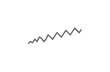
\begin{tikzpicture}[x=0.08em, y=0.08em, line width=0.4pt]
                \draw[FooterGray] (0,3) -- (1,4) -- (2,3.5) -- (3,5) -- (4,4) -- (5,6) -- (6,5.5) -- (7,4) -- (8,5) -- (9,7) -- (10,6) -- (11,5) -- (12,6.5) -- (13,8) -- (14,7) -- (15,6) -- (16,7.5) -- (17,9) -- (18,8) -- (19,7) -- (20,8.5) -- (21,10) -- (22,9) -- (23,8) -- (24,9.5);
            \end{tikzpicture}%
        }%
        \hskip0.5cm%
    }%
    \vskip6pt%
}

%=============================================================================
% PACKAGES
%=============================================================================
\usepackage[utf8]{inputenc}
\usepackage[T1]{fontenc}
\usepackage{amsmath, amssymb, amsthm}
\usepackage{mathtools}
\usepackage{bm}
\usepackage{tikz}
\usetikzlibrary{arrows.meta, positioning, shapes, calc, decorations.pathreplacing, shadings}
\usepackage{booktabs}
\usepackage{multirow}
\usepackage{array}
\usepackage{graphicx}
\usepackage{hyperref}
\usepackage{colortbl}
\hypersetup{colorlinks=true, linkcolor=MainBlue, urlcolor=MainBlue}
\graphicspath{{../../logos/}{../../charts/}{../../photos/}}
\hfuzz=2pt  % Suppress tiny overfull warnings (<2pt)
\vfuzz=2pt  % Suppress tiny vertical overfull warnings (<2pt)

%=============================================================================
% QUANTLET COMMAND
%=============================================================================
\newcommand{\quantlet}[2]{%
    \hfill\href{#2}{%
        \raisebox{-0.15em}{\includegraphics[height=0.7em]{ql_logo.png}}%
        \textcolor{MainBlue}{\tiny\ #1}%
    }%
}

%=============================================================================
% CUSTOM TITLE PAGE
%=============================================================================
\defbeamertemplate*{title page}{hybrid}[1][]
{
    \vspace{0.2cm}
    % Logos row - top header (with clickable links)
    \begin{center}
        \href{https://www.ase.ro}{\includegraphics[height=1.0cm]{ase_logo.png}}\hspace{0.3cm}%
        \href{https://theida.net}{\includegraphics[height=1.0cm]{ida_logo.png}}\hspace{0.3cm}%
        \href{https://blockchain-research-center.com}{\includegraphics[height=1.0cm]{brc_logo.png}}\hspace{0.3cm}%
        \href{https://www.ai4efin.ase.ro}{\includegraphics[height=1.0cm]{ai4efin_logo.png}}\hspace{0.3cm}%
        \href{https://ipe.ro/new}{\includegraphics[height=1.0cm]{acad_logo.png}}\hspace{0.3cm}%
        \href{https://www.digital-finance-msca.com}{\includegraphics[height=1.0cm]{msca_logo.png}}%
    \end{center}

    \vspace{0.6cm}

    % Main title with Q logos on sides (with clickable links)
    \begin{center}
        \begin{minipage}{0.1\textwidth}
            \centering
            \href{https://quantlet.com}{\includegraphics[height=1.1cm]{ql_logo.png}}
        \end{minipage}%
        \begin{minipage}{0.78\textwidth}
            \centering
            {\LARGE\bfseries\usebeamercolor[fg]{title}\inserttitle}

            \vspace{0.3cm}

            {\usebeamerfont{subtitle}\usebeamercolor[fg]{title}\insertsubtitle}
        \end{minipage}%
        \begin{minipage}{0.1\textwidth}
            \centering
            \href{https://quantinar.com}{\includegraphics[height=1.1cm]{qr_logo.png}}
        \end{minipage}
    \end{center}

    \vspace{0.6cm}

    % Authors (left aligned)
    \hspace{0.5cm}{\usebeamerfont{author}\insertauthor}

    \vspace{0.3cm}

    % Institute/Affiliations (left aligned)
    \hspace{0.5cm}\begin{minipage}[t]{0.9\textwidth}
        \raggedright\small\insertinstitute
    \end{minipage}
}

%=============================================================================
% THEOREM ENVIRONMENTS
%=============================================================================
\theoremstyle{definition}
\setbeamertemplate{theorems}[numbered]
\newtheorem{defn}{Definition}
\newtheorem{thm}{Theorem}
\newtheorem{prop}{Proposition}
\newtheorem{rmk}{Remark}

%=============================================================================
% CUSTOM COMMANDS
%=============================================================================
\newcommand{\E}{\mathbb{E}}
\newcommand{\Var}{\text{Var}}
\newcommand{\Cov}{\text{Cov}}
\newcommand{\Corr}{\text{Corr}}
\newcommand{\R}{\mathbb{R}}
\newcommand{\N}{\mathbb{N}}
\newcommand{\Z}{\mathbb{Z}}
\newcommand{\B}{\mathbf{B}}
\newcommand{\imark}{\textcolor{MainBlue}{\textbullet}}
\newcommand{\RMSE}{\text{RMSE}}
\newcommand{\MAE}{\text{MAE}}
\newcommand{\MAPE}{\text{MAPE}}

%=============================================================================
% TITLE INFORMATION
%=============================================================================
\title[Time Series Analysis]{Time Series Analysis and Forecasting}
\subtitle{Chapter 3: ARIMA Models}
\author[D.T. Pele]{Daniel Traian PELE}
\institute{Bucharest University of Economic Studies\\
IDA Institute Digital Assets\\
Blockchain Research Center\\
AI4EFin Artificial Intelligence for Energy Finance\\
Romanian Academy, Institute for Economic Forecasting\\
MSCA Digital Finance}
\date{}

%=============================================================================
%=============================================================================
% CENTRED MINIPAGE
%=============================================================================
\newenvironment{cminipage}[1]{%
    \par\noindent\hfill\begin{minipage}{#1}\ignorespaces
}{%
    \end{minipage}\hfill\null\par
}

\begin{document}

% Title page (no header/footer)
{
\setbeamertemplate{headline}{}
\setbeamertemplate{footline}{}
\begin{frame}[plain]
    \titlepage
\end{frame}
}

%=============================================================================
% LEARNING OBJECTIVES
%=============================================================================
\begin{frame}{Learning Objectives}
    \begin{cminipage}{0.95\textwidth}
    {\small
\begin{block}{By the end of this chapter, you will be able to:}
\begin{itemize}\setlength{\itemsep}{0pt}
    \item Understand the concept and implications of non-stationarity
    \item Apply differencing to achieve stationarity in time series
    \item Use the Augmented Dickey-Fuller (ADF) test for unit root detection
    \item Build, estimate, and forecast with ARIMA models
\end{itemize}
\end{block}
    }
    \end{cminipage}
\end{frame}

\begin{frame}{Data Sources and Software Tools}
    \begin{cminipage}{0.95\textwidth}
    \begin{columns}[T]
        \begin{column}{0.48\textwidth}
            \begin{block}{Data Sources}
                \begin{itemize}\setlength{\itemsep}{0pt}
                    \item \textbf{FRED} (Federal Reserve)
                    \begin{itemize}\setlength{\itemsep}{0pt}
                        \item US Real GDP (GDPC1), interest rates
                    \end{itemize}
                    \item \textbf{Yahoo Finance}
                    \begin{itemize}\setlength{\itemsep}{0pt}
                        \item Stock prices, exchange rates
                    \end{itemize}
                    \item \textbf{Eurostat / World Bank}
                    \begin{itemize}\setlength{\itemsep}{0pt}
                        \item Macroeconomic data
                    \end{itemize}
                    \item \textbf{Statsmodels datasets}
                    \begin{itemize}\setlength{\itemsep}{0pt}
                        \item Sunspots, Nile, Macrodata
                    \end{itemize}
                \end{itemize}
            \end{block}
        \end{column}
        \begin{column}{0.48\textwidth}
            \begin{exampleblock}{Python}
                \begin{itemize}\setlength{\itemsep}{0pt}
                    \item \texttt{statsmodels} --- ARIMA models
                    \item \texttt{pmdarima} --- automatic selection
                    \item \texttt{pandas-datareader} --- FRED download
                    \item \texttt{matplotlib} --- visualization
                    \item \texttt{scipy} --- statistical tests
                \end{itemize}
            \end{exampleblock}
            \begin{alertblock}{Resources}
                \begin{itemize}\setlength{\itemsep}{0pt}
                    \item \href{https://github.com/QuantLet/TSA/tree/main/TSA_ch3}{\texttt{github.com/QuantLet/TSA/TSA\_ch3}}
                    \item \href{https://quantlet.com}{\texttt{quantlet.com}}
                \end{itemize}
            \end{alertblock}
        \end{column}
    \end{columns}
    \end{cminipage}
\end{frame}

%=============================================================================
% TABLE OF CONTENTS
%=============================================================================
\begin{frame}{Chapter Outline}
    \begin{cminipage}{0.95\textwidth}
    \setbeamertemplate{section in toc}{\color{MainBlue}$\boxdot$~\inserttocsection}
    \tableofcontents
    \end{cminipage}
\end{frame}

%=============================================================================
% MOTIVATION
%=============================================================================
\section{Motivation}

\begin{frame}{Motivating Example: Non-Stationary Data Is Everywhere}
    \vspace{-0.2cm}
    \begin{center}
        \includegraphics[width=0.95\textwidth, height=0.55\textheight, keepaspectratio]{ch3_motivation_nonstationary.pdf}
    \end{center}
    \vspace{-0.2cm}
    {\footnotesize
    \begin{block}{Key Observations}
        \begin{itemize}\setlength{\itemsep}{0pt}
            \item Stock prices, GDP, exchange rates all exhibit \textbf{trends} or \textbf{wandering behavior}
            \item The sample mean (red line) is meaningless for a random walk
            \item Standard ARMA models \textbf{cannot} handle these series directly
        \end{itemize}
    \end{block}
    }
    \quantlet{TSA\_ch3\_motivation\_nonstationary}{https://github.com/QuantLet/TSA/tree/main/TSA_ch3/TSA_ch3_motivation_nonstationary}
\end{frame}

\begin{frame}{Real-World Applications}
    \vspace{-0.2cm}
    \begin{center}
        \includegraphics[width=0.95\textwidth, height=0.55\textheight, keepaspectratio]{ch3_motivation_realworld.pdf}
    \end{center}
    \vspace{-0.2cm}
    {\footnotesize
    \begin{alertblock}{The Challenge}
        Financial/economic data are typically I(1): stock prices, exchange rates, interest rates.
    \end{alertblock}
    }
    \quantlet{TSA\_ch3\_motivation\_realworld}{https://github.com/QuantLet/TSA/tree/main/TSA_ch3/TSA_ch3_motivation_realworld}
\end{frame}

\begin{frame}{The Solution: Differencing}
    \vspace{-0.2cm}
    \begin{center}
        \includegraphics[width=0.95\textwidth, height=0.55\textheight, keepaspectratio]{ch3_motivation_differencing.pdf}
    \end{center}
    \vspace{-0.2cm}
    {\footnotesize
    \begin{exampleblock}{Key Insight}
        \textbf{Differencing} transforms a non-stationary series into a stationary one:
        $\Delta Y_t = Y_t - Y_{t-1}$. The ACF changes from slow decay to quick decay!
    \end{exampleblock}
    }
    \quantlet{TSA\_ch3\_motivation\_differencing}{https://github.com/QuantLet/TSA/tree/main/TSA_ch3/TSA_ch3_motivation_differencing}
\end{frame}

\begin{frame}{What We'll Learn Today}
    \begin{cminipage}{0.95\textwidth}
    \begin{block}{Core Concepts}
        \begin{enumerate}
            \item \textbf{Non-Stationarity}: Why it matters and how to detect it
            \item \textbf{Unit Root Tests}: ADF, PP, KPSS tests
            \item \textbf{Differencing}: The key transformation
            \item \textbf{ARIMA Models}: Combining differencing with ARMA
            \item \textbf{Box-Jenkins Methodology}: Identify $\to$ Estimate $\to$ Diagnose
        \end{enumerate}
    \end{block}

    \vspace{0.2cm}

    \begin{exampleblock}{By the End of This Lecture}
        You will be able to model and forecast non-stationary time series like stock prices, GDP, and exchange rates using ARIMA models.
    \end{exampleblock}
    \end{cminipage}
\end{frame}

%=============================================================================
% SECTION 1: NON-STATIONARITY
%=============================================================================
\section{Non-Stationarity in Time Series}

\begin{frame}{Why Non-Stationarity Matters}
    \begin{cminipage}{0.95\textwidth}
    {\small
    \begin{alertblock}{The Problem}
        Many economic and financial time series are \textbf{non-stationary}:
        \begin{itemize}\setlength{\itemsep}{0pt}
            \item GDP, stock prices, exchange rates, inflation indices
            \item They exhibit trends, changing means, or growing variance
        \end{itemize}
    \end{alertblock}

    \vspace{0.1cm}

    \begin{block}{Consequences of Non-Stationarity}
        \begin{itemize}\setlength{\itemsep}{0pt}
            \item Standard ARMA models assume stationarity
            \item OLS regression with non-stationary data leads to \textbf{spurious regression}
            \item Sample moments (mean, variance, ACF) are not consistent estimators
            \item Statistical inference becomes invalid
        \end{itemize}
    \end{block}
    }
    \end{cminipage}
\end{frame}

\begin{frame}{Example: US Real GDP}
    \vspace{-0.2cm}
    \begin{center}
        \includegraphics[width=0.95\textwidth, height=0.55\textheight, keepaspectratio]{ch3_gdp_levels.pdf}
    \end{center}
    \vspace{-0.2cm}
    {\footnotesize
    \begin{block}{Key Observations}
        \begin{itemize}\setlength{\itemsep}{0pt}
            \item Clear upward \textbf{trend} -- mean is not constant
            \item This is a classic example of a \textbf{non-stationary} time series
            \item We cannot apply ARMA models directly to this data
        \end{itemize}
    \end{block}
    }
    \quantlet{TSA\_ch3\_gdp\_levels}{https://github.com/QuantLet/TSA/tree/main/TSA_ch3/TSA_ch3_gdp_levels}
\end{frame}

\begin{frame}{Types of Non-Stationarity}
    \begin{cminipage}{0.95\textwidth}
    \begin{columns}[T]
        \begin{column}{0.48\textwidth}
            \begin{block}{Deterministic Trend}
                $$Y_t = \alpha + \beta t + \varepsilon_t$$
                \begin{itemize}\setlength{\itemsep}{0pt}
                    \item Trend is a deterministic function of time
                    \item Can be removed by \textbf{detrending}
                    \item Shocks have temporary effects
                \end{itemize}
            \end{block}
        \end{column}
        \begin{column}{0.48\textwidth}
            \begin{block}{Stochastic Trend (Unit Root)}
                $$Y_t = Y_{t-1} + \varepsilon_t$$
                \begin{itemize}\setlength{\itemsep}{0pt}
                    \item Random walk process
                    \item Must be removed by \textbf{differencing}
                    \item Shocks have permanent effects
                \end{itemize}
            \end{block}
        \end{column}
    \end{columns}

    \vspace{0.3cm}

    \begin{alertblock}{Key Distinction}
        Correct identification is crucial: detrending a unit root $\rightarrow$ misspecification; differencing trend-stationary $\rightarrow$ misspecification.
    \end{alertblock}
    \end{cminipage}
\end{frame}

\begin{frame}{Visualizing the Difference}
    \vspace{-0.2cm}
    \begin{center}
        \includegraphics[width=0.95\textwidth, height=0.55\textheight, keepaspectratio]{ch3_trend_comparison.pdf}
    \end{center}
    \vspace{-0.2cm}
    {\footnotesize
    \begin{block}{Key Distinction}
        \begin{itemize}\setlength{\itemsep}{0pt}
            \item \textbf{Left}: Deterministic trend -- deviations from trend are temporary
            \item \textbf{Right}: Stochastic trend -- shocks accumulate permanently
            \item Both look similar, but require \textbf{different} treatments!
        \end{itemize}
    \end{block}
    }
    \quantlet{TSA\_ch3\_trend\_comparison}{https://github.com/QuantLet/TSA/tree/main/TSA_ch3/TSA_ch3_trend_comparison}
\end{frame}

\begin{frame}{The Random Walk Process}
    \begin{cminipage}{0.95\textwidth}
    {\small
    \begin{defn}[Random Walk]
        A \textbf{random walk} is defined as:
        $$Y_t = Y_{t-1} + \varepsilon_t, \quad \varepsilon_t \sim WN(0, \sigma^2)$$
        With initial condition $Y_0 = 0$, we have: $Y_t = \sum_{i=1}^{t} \varepsilon_i$
    \end{defn}

    \vspace{0.1cm}

    \begin{block}{Properties of Random Walk}
        \begin{itemize}\setlength{\itemsep}{0pt}
            \item $\E[Y_t] = 0$ (constant mean)
            \item $\Var(Y_t) = t\sigma^2$ (variance grows with time!)
            \item $\Cov(Y_t, Y_{t-k}) = (t-k)\sigma^2$ for $k \leq t$
            \item ACF: $\rho_k = \sqrt{\frac{t-k}{t}} \to 1$ as $t \to \infty$
        \end{itemize}
    \end{block}
    }
    \end{cminipage}
\end{frame}

\begin{frame}{Random Walk: Visual Illustration}
    \vspace{-0.2cm}
    \begin{center}
        \includegraphics[width=0.95\textwidth, height=0.55\textheight, keepaspectratio]{ch3_def_random_walk.pdf}
    \end{center}
    \vspace{-0.2cm}
    {\footnotesize
    \begin{alertblock}{Key Properties}
        \textbf{Left}: Paths wander unpredictably, no mean reversion.
        \textbf{Right}: $\Var(Y_t) = t\sigma^2$ grows linearly $\Rightarrow$ non-stationary.
    \end{alertblock}
    }
    \quantlet{TSA\_ch3\_def\_random\_walk}{https://github.com/QuantLet/TSA/tree/main/TSA_ch3/TSA_ch3_def_random_walk}
\end{frame}

\begin{frame}{Proof: Random Walk Variance}
    \begin{cminipage}{0.95\textwidth}
    {\small
    \textbf{Claim:} For $Y_t = Y_{t-1} + \varepsilon_t$ with $Y_0 = 0$: $\Var(Y_t) = t\sigma^2$

    \vspace{0.15cm}
    \textbf{Proof:} By recursive substitution: $Y_t = \sum_{i=1}^{t} \varepsilon_i$

    Taking variance:
    $$\Var(Y_t) = \Var\left(\sum_{i=1}^{t} \varepsilon_i\right) = \sum_{i=1}^{t} \Var(\varepsilon_i) + 2\sum_{i<j} \Cov(\varepsilon_i, \varepsilon_j)$$

    Since $\varepsilon_t$ independent (white noise): $\Var(Y_t) = \sum_{i=1}^{t} \sigma^2 = \boxed{t\sigma^2}$
    \begin{alertblock}{Variance depends on $t$ $\Rightarrow$ non-stationary}
    \end{alertblock}
    }
    \end{cminipage}
\end{frame}

\begin{frame}{Proof: Random Walk Autocovariance}
    \begin{cminipage}{0.95\textwidth}
    {\small
    \textbf{Claim:} $\Cov(Y_t, Y_{t-k}) = (t-k)\sigma^2$ for $k \leq t$

    \vspace{0.2cm}
    \textbf{Proof:} Using $Y_t = \sum_{i=1}^{t} \varepsilon_i$ and $Y_{t-k} = \sum_{i=1}^{t-k} \varepsilon_i$:
    \begin{align*}
    \Cov(Y_t, Y_{t-k}) &= \Cov\left(\sum_{i=1}^{t} \varepsilon_i, \sum_{j=1}^{t-k} \varepsilon_j\right) \\
    &= \sum_{i=1}^{t}\sum_{j=1}^{t-k} \Cov(\varepsilon_i, \varepsilon_j) = \sum_{i=1}^{t-k} \Var(\varepsilon_i) = \boxed{(t-k)\sigma^2}
    \end{align*}

    Only terms with $i = j$ survive (when $i \leq t-k$).

    \vspace{0.1cm}
    \textbf{ACF:}
    $$\rho(k) = \frac{\Cov(Y_t, Y_{t-k})}{\sqrt{\Var(Y_t)\Var(Y_{t-k})}} = \frac{(t-k)\sigma^2}{\sqrt{t\sigma^2 \cdot (t-k)\sigma^2}} = \sqrt{\frac{t-k}{t}}$$
    }
    \end{cminipage}
\end{frame}

\begin{frame}{Random Walk with Drift}
    \begin{cminipage}{0.95\textwidth}
    {\small
    \begin{defn}[Random Walk with Drift]
        A random walk with drift includes a constant term:
        $$Y_t = \mu + Y_{t-1} + \varepsilon_t$$
        Equivalently: $Y_t = Y_0 + \mu t + \sum_{i=1}^{t} \varepsilon_i$
    \end{defn}

    \vspace{0.1cm}

    \begin{block}{Properties}
        \begin{itemize}\setlength{\itemsep}{0pt}
            \item $\E[Y_t] = Y_0 + \mu t$ (mean grows linearly)
            \item $\Var(Y_t) = t\sigma^2$ (variance still grows)
            \item The drift $\mu$ creates an upward or downward trend
            \item Still non-stationary despite having a ``trend''
        \end{itemize}
    \end{block}
    }
    \end{cminipage}
\end{frame}

\begin{frame}{Random Walk with Drift: Visual Illustration}
    \vspace{-0.2cm}
    \begin{center}
        \includegraphics[width=0.95\textwidth, height=0.55\textheight, keepaspectratio]{ch3_def_random_walk_drift.pdf}
    \end{center}
    \vspace{-0.2cm}
    {\footnotesize
    \begin{exampleblock}{Comparison}
        Without drift (blue): wanders around zero with no direction. With drift $\mu > 0$ (red): systematic upward trend. Both are non-stationary --- drift adds deterministic trend to stochastic wandering.
    \end{exampleblock}
    }
    \quantlet{TSA\_ch3\_def\_random\_walk\_drift}{https://github.com/QuantLet/TSA/tree/main/TSA_ch3/TSA_ch3_def_random_walk_drift}
\end{frame}

\begin{frame}{Simulating Random Walks}
    \vspace{-0.2cm}
    \begin{center}
        \includegraphics[width=0.95\textwidth, height=0.55\textheight, keepaspectratio]{ch3_random_walk.pdf}
    \end{center}
    \vspace{-0.2cm}
    {\footnotesize
    \begin{block}{Random Walk Types}
        \begin{itemize}\setlength{\itemsep}{0pt}
            \item \textbf{Left}: Pure random walks -- no drift, wander unpredictably
            \item \textbf{Right}: Random walks with drift -- upward trend on average
            \item Each path is unique; uncertainty grows over time
        \end{itemize}
    \end{block}
    }
    \quantlet{TSA\_ch3\_random\_walk}{https://github.com/QuantLet/TSA/tree/main/TSA_ch3/TSA_ch3_random_walk}
\end{frame}

\begin{frame}{Variance Growth: Why Random Walks Are Non-Stationary}
    \vspace{-0.2cm}
    \begin{center}
        \includegraphics[width=0.95\textwidth, height=0.51\textheight, keepaspectratio]{ch3_variance_growth.pdf}
    \end{center}
    \vspace{-0.2cm}
    {\footnotesize
    \begin{block}{Key Observations}
        \begin{itemize}\setlength{\itemsep}{0pt}
            \item \textbf{Left}: Fan of paths shows uncertainty growing over time
            \item \textbf{Right}: Variance grows linearly: $\Var(Y_t) = t\sigma^2$
            \item This violates stationarity (variance should be constant)
        \end{itemize}
    \end{block}
    }
    \quantlet{TSA\_ch3\_variance\_growth}{https://github.com/QuantLet/TSA/tree/main/TSA_ch3/TSA_ch3_variance_growth}
\end{frame}

\begin{frame}{Integrated Processes}
    \begin{cminipage}{0.95\textwidth}
    {\small
    \begin{defn}[Integrated Process of Order $d$]
        A time series $\{Y_t\}$ is \textbf{integrated of order $d$}, written $Y_t \sim I(d)$, if:
        \begin{itemize}\setlength{\itemsep}{0pt}
            \item $Y_t$ is non-stationary
            \item $(1-L)^d Y_t = \Delta^d Y_t$ is stationary
            \item $(1-L)^{d-1} Y_t$ is still non-stationary
        \end{itemize}
    \end{defn}

    \vspace{0.1cm}

    \begin{exampleblock}{Common Cases}
        \begin{itemize}\setlength{\itemsep}{0pt}
            \item $I(0)$: Stationary process (e.g., ARMA)
            \item $I(1)$: First difference is stationary (most common for economic data)
            \item $I(2)$:
                \begin{itemize}\setlength{\itemsep}{0pt}
                    \item Second difference is stationary (less common)
                \end{itemize}
            \end{itemize}
    \end{exampleblock}
    }
    \end{cminipage}
\end{frame}

\begin{frame}{Integrated Process: Visual Illustration}
    \vspace{-0.2cm}
    \begin{center}
        \includegraphics[width=0.95\textwidth, height=0.48\textheight, keepaspectratio]{ch3_def_integrated.pdf}
    \end{center}
    \vspace{-0.2cm}
    {\footnotesize
    \begin{block}{Order of Integration}
        \begin{itemize}\setlength{\itemsep}{0pt}
            \item $I(0)$: Stationary $\Rightarrow$ no differencing needed
            \item $I(1)$: One difference needed (random walk)
            \item $I(2)$: Two differences needed
            \item Most economic series are $I(0)$ or $I(1)$
        \end{itemize}
    \end{block}
    }
    \quantlet{TSA\_ch3\_def\_integrated}{https://github.com/QuantLet/TSA/tree/main/TSA_ch3/TSA_ch3_def_integrated}
\end{frame}

%=============================================================================
% SECTION 2: DIFFERENCING
%=============================================================================
\section{Differencing and the Difference Operator}

\begin{frame}{The Difference Operator}
    \begin{cminipage}{0.95\textwidth}
    {\small
    \begin{defn}[First Difference]
        The \textbf{first difference operator} $\Delta$ is defined as:
        $\Delta Y_t = Y_t - Y_{t-1} = (1-L)Y_t$, where $L$ is the lag operator ($LY_t = Y_{t-1}$).
    \end{defn}

    \vspace{0.1cm}

    \begin{block}{Higher-Order Differences}
        \begin{itemize}\setlength{\itemsep}{0pt}
            \item Second difference: $\Delta^2 Y_t = \Delta(\Delta Y_t) = (1-L)^2 Y_t$
            \item $\Delta^2 Y_t = Y_t - 2Y_{t-1} + Y_{t-2}$
            \item $d$-th difference: $\Delta^d Y_t = (1-L)^d Y_t$
        \end{itemize}
    \end{block}

    \vspace{0.1cm}

    \begin{alertblock}{Key Result}
        If $Y_t \sim I(d)$, then $\Delta^d Y_t \sim I(0)$ (stationary).
    \end{alertblock}
    }
    \end{cminipage}
\end{frame}

\begin{frame}{First Difference: Visual Illustration}
    \vspace{-0.2cm}
    \begin{center}
        \includegraphics[width=0.95\textwidth, height=0.55\textheight, keepaspectratio]{ch3_def_difference.pdf}
    \end{center}
    \vspace{-0.2cm}
    {\footnotesize
    \begin{block}{Observation}
        \begin{itemize}\setlength{\itemsep}{0pt}
            \item \textbf{Left}: non-stationary series
            \item \textbf{Right}: after first difference, the series becomes stationary
        \end{itemize}
    \end{block}
    }
    \quantlet{TSA\_ch3\_def\_difference}{https://github.com/QuantLet/TSA/tree/main/TSA_ch3/TSA_ch3_def_difference}
\end{frame}

\begin{frame}{Example: Differencing a Random Walk}
    \begin{cminipage}{0.95\textwidth}
    {\small
    \begin{exampleblock}{Random Walk to White Noise}
        Let $Y_t = Y_{t-1} + \varepsilon_t$ (random walk). Taking the first difference:
        $$\Delta Y_t = Y_t - Y_{t-1} = \varepsilon_t$$
        The first difference is white noise -- a stationary process!
    \end{exampleblock}

    \vspace{0.1cm}

    \begin{block}{Interpretation}
        \begin{itemize}\setlength{\itemsep}{0pt}
            \item A random walk is $I(1)$
            \item One difference transforms it to $I(0)$
            \item The ``changes'' in a random walk are stationary
        \end{itemize}
    \end{block}
    }
    \end{cminipage}
\end{frame}

\begin{frame}{Proof: Differencing Induces Stationarity}
    \begin{cminipage}{0.95\textwidth}
    {\small
    \textbf{Claim:} If $Y_t \sim I(1)$, then $\Delta Y_t = Y_t - Y_{t-1}$ is stationary.

    \vspace{0.15cm}
    \textbf{Proof for Random Walk with Drift:} $Y_t = \mu + Y_{t-1} + \varepsilon_t$

    The first difference is:
    $$\Delta Y_t = Y_t - Y_{t-1} = \mu + \varepsilon_t$$

    Check stationarity conditions:
    \begin{enumerate}\setlength{\itemsep}{0pt}
        \item \textbf{Mean:} $\E[\Delta Y_t] = \mu$ (constant, does not depend on $t$) \checkmark
        \item \textbf{Variance:} $\Var(\Delta Y_t) = \Var(\varepsilon_t) = \sigma^2$ (constant) \checkmark
        \item \textbf{Autocovariance:} $\Cov(\Delta Y_t, \Delta Y_{t-k}) = \Cov(\varepsilon_t, \varepsilon_{t-k}) = 0$ for $k \neq 0$ \checkmark
    \end{enumerate}

    \begin{exampleblock}{General Principle}
        Differencing removes the ``memory'' that causes variance to accumulate. For $I(d)$ processes, $d$ differences are needed.
    \end{exampleblock}
    }
    \end{cminipage}
\end{frame}

\begin{frame}{ACF Diagnostic: Detecting Non-Stationarity}
    \vspace{-0.2cm}
    \begin{center}
        \includegraphics[width=0.95\textwidth, height=0.55\textheight, keepaspectratio]{ch3_acf_nonstationary.pdf}
    \end{center}
    \vspace{-0.2cm}
    {\footnotesize
    \begin{block}{ACF Patterns}
        \begin{itemize}\setlength{\itemsep}{0pt}
            \item \textbf{Top}: Random walk ACF decays very slowly $\Rightarrow$ unit root
            \item \textbf{Bottom}: After differencing, ACF cuts off $\Rightarrow$ stationary
        \end{itemize}
    \end{block}
    }
    \quantlet{TSA\_ch3\_acf\_nonstationary}{https://github.com/QuantLet/TSA/tree/main/TSA_ch3/TSA_ch3_acf_nonstationary}
\end{frame}

\begin{frame}{Differencing in Practice: GDP Example}
    \vspace{-0.2cm}
    \begin{center}
        \includegraphics[width=0.95\textwidth, height=0.55\textheight, keepaspectratio]{ch3_differencing.pdf}
    \end{center}
    \vspace{-0.2cm}
    {\footnotesize
    \begin{block}{Transformation}
        \textbf{Left}: GDP in levels with clear upward trend (non-stationary). \textbf{Right}: GDP growth rate $\Delta \log(GDP_t)$ fluctuates around constant mean (stationary). One difference removes the stochastic trend.
    \end{block}
    }
    \quantlet{TSA\_ch3\_differencing}{https://github.com/QuantLet/TSA/tree/main/TSA_ch3/TSA_ch3_differencing}
\end{frame}

\begin{frame}{Overdifferencing}
    \begin{cminipage}{0.95\textwidth}
    {\small
    \begin{alertblock}{Warning: Overdifferencing}
        Differencing more than necessary introduces problems:
        \begin{itemize}\setlength{\itemsep}{2pt}
            \item Creates artificial negative autocorrelation
            \begin{itemize}\setlength{\itemsep}{0pt}
                \item ACF shows spurious patterns
            \end{itemize}
            \item Inflates variance
            \begin{itemize}\setlength{\itemsep}{0pt}
                \item Reduces forecast accuracy
            \end{itemize}
            \item Loses information
            \begin{itemize}\setlength{\itemsep}{0pt}
                \item Cannot recover original level
            \end{itemize}
        \end{itemize}
    \end{alertblock}

    \vspace{0.1cm}

    \begin{exampleblock}{Example}
        If $Y_t \sim I(1)$, then $\Delta Y_t \sim I(0)$. But if we difference again:
        $$\Delta^2 Y_t = \Delta Y_t - \Delta Y_{t-1} = \varepsilon_t - \varepsilon_{t-1}$$
        This is an MA(1) with $\theta = 1$ (non-invertible boundary)!
    \end{exampleblock}
    }
    \end{cminipage}
\end{frame}

%=============================================================================
% SECTION 3: ARIMA MODELS
%=============================================================================
\section{ARIMA(p,d,q) Models}

\begin{frame}{Definition of ARIMA}
    \begin{cminipage}{0.95\textwidth}
    {\small
    \begin{defn}[ARIMA(p,d,q)]
        A time series $\{Y_t\}$ follows an \textbf{ARIMA(p,d,q)} process if:
        $$\phi(L)(1-L)^d Y_t = c + \theta(L)\varepsilon_t$$
        where:
        \begin{itemize}\setlength{\itemsep}{0pt}
            \item $\phi(L) = 1 - \phi_1 L - \phi_2 L^2 - \cdots - \phi_p L^p$ (AR polynomial)
            \item $\theta(L) = 1 + \theta_1 L + \theta_2 L^2 + \cdots + \theta_q L^q$ (MA polynomial)
            \item $d$ is the order of integration (number of differences)
            \item $\varepsilon_t \sim WN(0, \sigma^2)$
        \end{itemize}
    \end{defn}
    }
    \end{cminipage}
\end{frame}

\begin{frame}{ARIMA: Visual Illustration}
    \vspace{-0.2cm}
    \begin{center}
        \includegraphics[width=0.95\textwidth, height=0.55\textheight, keepaspectratio]{ch3_def_arima.pdf}
    \end{center}
    \vspace{-0.2cm}
    {\footnotesize
    \begin{block}{Interpretation}
        Top: original ARIMA series (non-stationary). Bottom: after differencing $d$ times, ACF/PACF reveal the AR and MA orders for the stationary component.
    \end{block}
    }
    \quantlet{TSA\_ch3\_def\_arima}{https://github.com/QuantLet/TSA/tree/main/TSA_ch3/TSA_ch3_def_arima}
\end{frame}

\begin{frame}{ARIMA Components}
    \begin{cminipage}{0.95\textwidth}
    {\small
    \begin{center}
        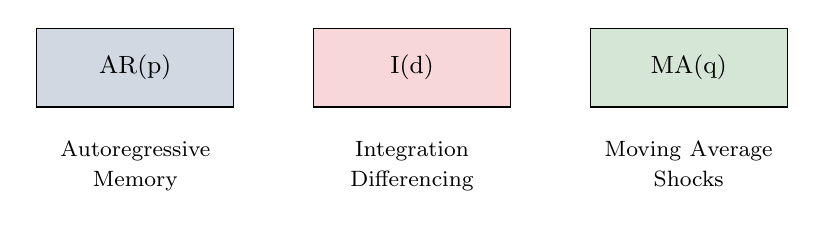
\begin{tikzpicture}[node distance=2cm, every node/.style={font=\small}]
            \node[draw, rectangle, fill=MainBlue!20, minimum width=2.5cm, minimum height=1cm] (AR) {AR(p)};
            \node[draw, rectangle, fill=Crimson!20, minimum width=2.5cm, minimum height=1cm, right=1cm of AR] (I) {I(d)};
            \node[draw, rectangle, fill=Forest!20, minimum width=2.5cm, minimum height=1cm, right=1cm of I] (MA) {MA(q)};

            \node[below=0.3cm of AR, text width=2.5cm, align=center] {\footnotesize Autoregressive\\Memory};
            \node[below=0.3cm of I, text width=2.5cm, align=center] {\footnotesize Integration\\Differencing};
            \node[below=0.3cm of MA, text width=2.5cm, align=center] {\footnotesize Moving Average\\Shocks};
        \end{tikzpicture}
    \end{center}

    \vspace{0.2cm}

    \begin{block}{Special Cases}
        \begin{itemize}\setlength{\itemsep}{0pt}
            \item ARIMA(p,0,q) = ARMA(p,q) -- stationary
            \item ARIMA(0,1,0) = Random walk
            \item ARIMA(0,1,1) = IMA(1,1) -- exponential smoothing
            \item ARIMA(1,1,0) = ARI(1,1) -- differenced AR(1)
        \end{itemize}
    \end{block}
    }
    \end{cminipage}
\end{frame}

\begin{frame}{ARIMA(1,1,0) Example}
    \begin{cminipage}{0.95\textwidth}
    {\small
    \begin{exampleblock}{ARI(1,1) Model}
        $$\Delta Y_t = c + \phi_1 \Delta Y_{t-1} + \varepsilon_t$$
        Equivalently: $(1-\phi_1 L)(1-L)Y_t = c + \varepsilon_t$
    \end{exampleblock}

    \vspace{0.1cm}

    \begin{block}{Interpretation}
        \begin{itemize}\setlength{\itemsep}{0pt}
            \item The \textbf{changes} in $Y_t$ follow an AR(1) process
            \item If $|\phi_1| < 1$, the changes are stationary
            \item $Y_t$ itself has a stochastic trend
            \item Common model for many economic time series
        \end{itemize}
    \end{block}
    }
    \end{cminipage}
\end{frame}

\begin{frame}{ARIMA(0,1,1) Example}
    \begin{cminipage}{0.95\textwidth}
    {\small
    \begin{exampleblock}{IMA(1,1) Model}
        $$\Delta Y_t = c + \varepsilon_t + \theta_1 \varepsilon_{t-1}$$
        Equivalently: $(1-L)Y_t = c + (1+\theta_1 L)\varepsilon_t$
    \end{exampleblock}

    \vspace{0.1cm}

    \begin{block}{Connection to Exponential Smoothing}
        The IMA(1,1) model is equivalent to \textbf{simple exponential smoothing}:
        $$\hat{Y}_{t+1} = \alpha Y_t + (1-\alpha)\hat{Y}_t$$
        where $\alpha = 1 + \theta_1$ (for $-1 < \theta_1 < 0$).
    \end{block}
    }
    \end{cminipage}
\end{frame}

\begin{frame}{The Role of the Constant in ARIMA}
    \begin{cminipage}{0.95\textwidth}
    {\small
    \begin{block}{Constant Term in ARIMA(p,d,q)}
        When $d > 0$, the constant $c$ has a different interpretation:
        $\phi(L)(1-L)^d Y_t = c + \theta(L)\varepsilon_t$
    \end{block}

    \vspace{0.1cm}

    \begin{alertblock}{Important Implications}
        \begin{itemize}\setlength{\itemsep}{2pt}
            \item For $d=1$: $c$ represents the \textbf{drift}
            \begin{itemize}\setlength{\itemsep}{0pt}
                \item Average change: $\E[\Delta Y_t] = \frac{c}{1-\phi_1-\cdots-\phi_p}$
                \item Linear trend in levels
            \end{itemize}
            \item For $d=2$: $c$ affects the \textbf{curvature}
            \begin{itemize}\setlength{\itemsep}{0pt}
                \item Quadratic trend in levels
            \end{itemize}
            \item Often $c=0$ is assumed when $d \geq 1$
            \begin{itemize}\setlength{\itemsep}{0pt}
                \item No deterministic trend component
            \end{itemize}
        \end{itemize}
    \end{alertblock}
    }
    \end{cminipage}
\end{frame}

%=============================================================================
% SECTION 4: UNIT ROOT TESTS
%=============================================================================
\section{Unit Root Tests}

\begin{frame}{Testing for Unit Roots}
    \begin{cminipage}{0.95\textwidth}
    {\small
    \begin{block}{Why Test?}
        Before fitting an ARIMA model, we need to determine:
        \begin{enumerate}\setlength{\itemsep}{0pt}
            \item Is the series stationary? (Is $d=0$?)
            \item If not, how many differences are needed? (What is $d$?)
        \end{enumerate}
    \end{block}

    \vspace{0.1cm}

    \begin{block}{Common Unit Root Tests}
        \begin{itemize}\setlength{\itemsep}{0pt}
            \item \textbf{Dickey-Fuller (DF)} and \textbf{Augmented Dickey-Fuller (ADF)}
            \item \textbf{Phillips-Perron (PP)}
            \item \textbf{KPSS} (stationarity test -- reversed null hypothesis)
        \end{itemize}
    \end{block}
    }
    \end{cminipage}
\end{frame}

\begin{frame}{Researcher Spotlight: Dickey \& Fuller}
    \vspace{-0.2cm}
    \begin{columns}[T]
        \begin{column}{0.22\textwidth}
            \centering
            \includegraphics[width=0.95\textwidth, height=0.22\textheight, keepaspectratio]{photo_david_dickey.jpg}
            \\[0.05cm]
            {\tiny\textcolor{MediumGray}{David Dickey (*1945)}}\\[0.02cm]
            \href{https://en.wikipedia.org/wiki/David_Dickey}{\faWikipediaW\ \textcolor{MainBlue}{\tiny Wikipedia}}
        \end{column}
        \begin{column}{0.76\textwidth}
            \begin{block}{Biography}
                {\footnotesize \begin{itemize}\setlength{\itemsep}{0pt}
                    \item \textbf{David Dickey}: American statistician at NC State University. PhD student of Wayne Fuller at Iowa State
                    \item \textbf{Wayne Fuller}: American statistician, professor at Iowa State University
                    \item Together they developed the foundational test for unit roots in time series
                \end{itemize}}
            \end{block}
        \end{column}
    \end{columns}
    \vspace{0.1cm}
    \begin{columns}[T]
        \begin{column}{0.22\textwidth}
            \centering
            \includegraphics[width=0.95\textwidth, height=0.22\textheight, keepaspectratio]{photo_wayne_fuller.jpg}
            \\[0.05cm]
            {\tiny\textcolor{MediumGray}{Wayne Fuller (1931--2022)}}\\[0.02cm]
            \href{https://en.wikipedia.org/wiki/Wayne_Fuller}{\faWikipediaW\ \textcolor{MainBlue}{\tiny Wikipedia}}
        \end{column}
        \begin{column}{0.76\textwidth}
            \begin{exampleblock}{Key Contributions}
                {\footnotesize \begin{itemize}\setlength{\itemsep}{0pt}
                    \item \textbf{Dickey-Fuller test} (1979) --- the fundamental unit root test
                    \item \textbf{Augmented Dickey-Fuller (ADF)} --- extension with lagged differences
                    \item \textbf{Critical value tables} --- non-standard distributions under the null
                    \item Enabled rigorous testing of integration order for ARIMA modeling
                \end{itemize}}
            \end{exampleblock}
        \end{column}
    \end{columns}
\end{frame}

\begin{frame}{The Dickey-Fuller Test}
    \begin{cminipage}{0.95\textwidth}
    {\small
    \begin{block}{Setup}
        Consider the AR(1) model: $Y_t = \phi Y_{t-1} + \varepsilon_t$. Subtract $Y_{t-1}$:
        $\Delta Y_t = (\phi - 1)Y_{t-1} + \varepsilon_t = \gamma Y_{t-1} + \varepsilon_t$, where $\gamma = \phi - 1$.
    \end{block}

    \vspace{0.1cm}

    \begin{block}{Hypotheses}
        \begin{itemize}\setlength{\itemsep}{0pt}
            \item $H_0$: $\gamma = 0$ (unit root, $\phi = 1$, non-stationary)
            \item $H_1$: $\gamma < 0$ (stationary, $|\phi| < 1$)
        \end{itemize}
    \end{block}

    \vspace{0.1cm}

    \begin{alertblock}{Key Issue}
        Under $H_0$, the $t$-statistic does \textbf{not} follow a standard $t$-distribution! Must use Dickey-Fuller critical values.
    \end{alertblock}
    }
    \end{cminipage}
\end{frame}

\begin{frame}{Dickey-Fuller Test Variants}
    \begin{cminipage}{0.95\textwidth}
    {\small
    \begin{block}{Three Specifications}
        \begin{enumerate}\setlength{\itemsep}{0pt}
            \item \textbf{No constant, no trend}: $\Delta Y_t = \gamma Y_{t-1} + \varepsilon_t$
            \item \textbf{With constant (drift)}: $\Delta Y_t = \alpha + \gamma Y_{t-1} + \varepsilon_t$
            \item \textbf{With constant and trend}: $\Delta Y_t = \alpha + \beta t + \gamma Y_{t-1} + \varepsilon_t$
        \end{enumerate}
    \end{block}

    \vspace{0.1cm}

    \begin{alertblock}{Choosing the Right Specification}
        \begin{itemize}\setlength{\itemsep}{0pt}
            \item Examine the data: does it have a visible trend?
            \item Including unnecessary terms reduces power
            \item Excluding necessary terms leads to incorrect inference
        \end{itemize}
    \end{alertblock}
    }
    \end{cminipage}
\end{frame}

\begin{frame}{Augmented Dickey-Fuller (ADF) Test}
    \begin{cminipage}{0.95\textwidth}
    {\small
    \begin{block}{The Problem with Simple DF}
        If AR dynamics beyond AR(1) exist, DF residuals will be autocorrelated.
    \end{block}

    \vspace{0.1cm}

    \begin{defn}[ADF Test]
        Add lagged differences: $\Delta Y_t = \alpha + \beta t + \gamma Y_{t-1} + \sum_{j=1}^{k} \delta_j \Delta Y_{t-j} + \varepsilon_t$

        Test $H_0: \gamma = 0$ using ADF critical values.
    \end{defn}

    \vspace{0.1cm}

    \begin{block}{Choosing Lag Length $k$}
        \begin{itemize}\setlength{\itemsep}{0pt}
            \item Use information criteria (AIC, BIC)
            \item Start with $k_{max}$, reduce until last lag significant
        \end{itemize}
    \end{block}
    }
    \end{cminipage}
\end{frame}

\begin{frame}{ADF Test: Visual Illustration}
    \vspace{-0.2cm}
    \begin{center}
        \includegraphics[width=0.95\textwidth, height=0.55\textheight, keepaspectratio]{ch3_def_adf.pdf}
    \end{center}
    \vspace{-0.2cm}
    {\footnotesize
    \begin{block}{Observation}
        \begin{itemize}\setlength{\itemsep}{0pt}
            \item \textbf{Left}: stationary series $\Rightarrow$ ADF rejects unit root
            \item \textbf{Right}: non-stationary $\Rightarrow$ ADF fails to reject
        \end{itemize}
    \end{block}
    }
    \quantlet{TSA\_ch3\_def\_adf}{https://github.com/QuantLet/TSA/tree/main/TSA_ch3/TSA_ch3_def_adf}
\end{frame}

\begin{frame}{ADF Test Critical Values}
    \begin{cminipage}{0.95\textwidth}
    {\small
    \begin{table}
        \centering
        \begin{tabular}{lccc}
            \toprule
            \textbf{Model} & \textbf{1\%} & \textbf{5\%} & \textbf{10\%} \\
            \midrule
            No constant, no trend & $-2.58$ & $-1.95$ & $-1.62$ \\
            With constant & $-3.43$ & $-2.86$ & $-2.57$ \\
            With constant and trend & $-3.96$ & $-3.41$ & $-3.13$ \\
            \bottomrule
        \end{tabular}
    \end{table}
    \begin{block}{Decision Rule}
        \begin{itemize}
            \item Test statistic $<$ critical value $\Rightarrow$ Reject $H_0$ (stationary)
            \item Test statistic $\geq$ critical value $\Rightarrow$ Fail to reject (unit root)
        \end{itemize}
    \end{block}
    }
    \end{cminipage}
\end{frame}

\begin{frame}{The Phillips-Perron (PP) Test}
    \begin{cminipage}{0.95\textwidth}
    {\small
    \begin{block}{Motivation}
        Like ADF, tests $H_0$: Unit root vs $H_1$: Stationary, but uses a \textbf{non-parametric correction} for serial correlation instead of adding lagged differences.
    \end{block}

    \begin{block}{Test Statistic}
        The PP test modifies the DF $t$-statistic:
        $$Z_t = t_{\hat{\gamma}} \cdot \sqrt{\frac{\hat{\sigma}^2}{\hat{\lambda}^2}} - \frac{T(\hat{\lambda}^2 - \hat{\sigma}^2)(se(\hat{\gamma}))}{2\hat{\lambda}^2 \cdot s}$$
        where $\hat{\lambda}^2$ is a consistent estimate of the long-run variance using Newey-West.
    \end{block}

    \begin{exampleblock}{Advantages over ADF}
        \begin{itemize}\setlength{\itemsep}{0pt}
            \item Robust to heteroskedasticity and serial correlation
            \item No need to select lag length (uses bandwidth instead)
        \end{itemize}
    \end{exampleblock}
    }
    \end{cminipage}
\end{frame}

\begin{frame}{The KPSS Test}
    \begin{cminipage}{0.95\textwidth}
    {\small
    \begin{block}{Reversed Hypotheses}
        Unlike ADF: $H_0$: Stationary \quad vs \quad $H_1$: Unit root
    \end{block}

    \vspace{0.1cm}

    \begin{block}{KPSS Procedure}
        Decompose: $Y_t = \xi t + r_t + \varepsilon_t$ where $r_t = r_{t-1} + u_t$.
        Test whether $\Var(u_t) = 0$.
    \end{block}

    \vspace{0.1cm}

    \begin{exampleblock}{Complementary Use with ADF}
        \begin{itemize}\setlength{\itemsep}{0pt}
            \item ADF rejects, KPSS doesn't $\Rightarrow$ Stationary
            \item ADF doesn't reject, KPSS rejects $\Rightarrow$ Unit root
            \item Both reject or neither $\Rightarrow$ Inconclusive
        \end{itemize}
    \end{exampleblock}
    }
    \end{cminipage}
\end{frame}

%=============================================================================
% SECTION 5: MODEL IDENTIFICATION
%=============================================================================
\section{ARIMA Model Identification}

\begin{frame}{The Box-Jenkins Methodology}
    \begin{cminipage}{0.95\textwidth}
    \begin{center}
        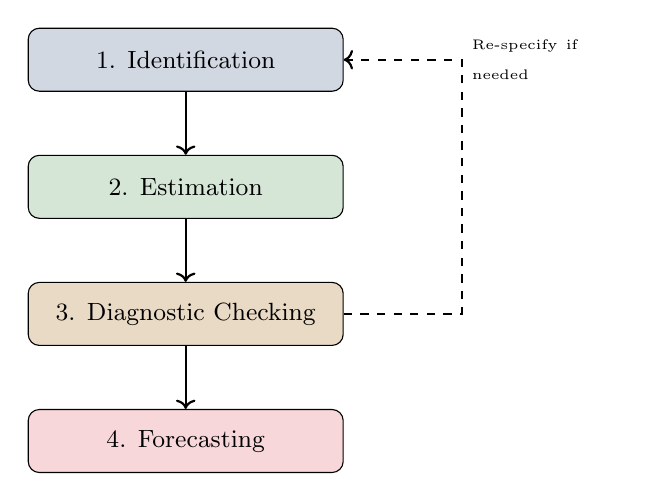
\begin{tikzpicture}[node distance=1.5cm, every node/.style={font=\small}]
            \node[draw, rectangle, rounded corners, fill=MainBlue!20, minimum width=4cm, minimum height=0.8cm] (id) {1. Identification};
            \node[draw, rectangle, rounded corners, fill=Forest!20, minimum width=4cm, minimum height=0.8cm, below=0.8cm of id] (est) {2. Estimation};
            \node[draw, rectangle, rounded corners, fill=Amber!30, minimum width=4cm, minimum height=0.8cm, below=0.8cm of est] (diag) {3. Diagnostic Checking};
            \node[draw, rectangle, rounded corners, fill=Crimson!20, minimum width=4cm, minimum height=0.8cm, below=0.8cm of diag] (fore) {4. Forecasting};

            \draw[->, thick] (id) -- (est);
            \draw[->, thick] (est) -- (diag);
            \draw[->, thick] (diag) -- (fore);
            \draw[->, thick, dashed] (diag.east) -- ++(1.5,0) |- (id.east) node[midway, right, text width=2cm] {\tiny Re-specify if needed};
        \end{tikzpicture}
    \end{center}
    \end{cminipage}
\end{frame}

\begin{frame}{Step 1: Determining $d$}
    \begin{cminipage}{0.95\textwidth}
    {\small
    \begin{block}{Procedure}
        \begin{enumerate}\setlength{\itemsep}{0pt}
            \item Plot the time series -- look for trends, changing variance
            \item Examine ACF -- slow decay suggests non-stationarity
            \item Apply unit root tests (ADF, KPSS)
            \item If non-stationary, difference and repeat
        \end{enumerate}
    \end{block}

    \vspace{0.1cm}

    \begin{exampleblock}{Practical Guidelines}
        \begin{itemize}\setlength{\itemsep}{0pt}
            \item Most economic series: $d = 1$ is sufficient
            \item Rarely need $d > 2$
            \item If ACF of $\Delta Y_t$ still decays slowly, try $d = 2$
            \item Watch for overdifferencing (ACF with $\rho_1 \approx -0.5$)
        \end{itemize}
    \end{exampleblock}
    }
    \end{cminipage}
\end{frame}

\begin{frame}{Step 2: Determining $p$ and $q$}
    \begin{cminipage}{0.95\textwidth}
    {\small
    \begin{block}{After Differencing}
        Once $W_t = \Delta^d Y_t$ is stationary, use ACF/PACF to identify ARMA($p$,$q$):
    \end{block}

    \vspace{0.1cm}

    \begin{center}
        \begin{tabular}{lcc}
            \toprule
            \textbf{Model} & \textbf{ACF} & \textbf{PACF} \\
            \midrule
            AR($p$) & Decays exponentially & Cuts off after lag $p$ \\
            MA($q$) & Cuts off after lag $q$ & Decays exponentially \\
            ARMA($p$,$q$) & Decays & Decays \\
            \bottomrule
        \end{tabular}
    \end{center}

    \vspace{0.1cm}

    \begin{block}{Information Criteria}
        When patterns are unclear, compare models using:
        \begin{itemize}\setlength{\itemsep}{0pt}
            \item AIC = $-2\ln(L) + 2k$; \quad BIC = $-2\ln(L) + k\ln(n)$
        \end{itemize}
        Lower is better. BIC penalizes complexity more.
    \end{block}
    }
    \end{cminipage}
\end{frame}

\begin{frame}{Auto-ARIMA Algorithms}
    \begin{cminipage}{0.95\textwidth}
    {\small
    \begin{block}{Automated Model Selection}
        Modern software can automatically select $(p,d,q)$:
        \begin{itemize}\setlength{\itemsep}{0pt}
            \item Python: \texttt{pmdarima.auto\_arima()}
            \item R: \texttt{forecast::auto.arima()}
        \end{itemize}
    \end{block}

    \vspace{0.1cm}

    \begin{block}{How Auto-ARIMA Works}
        \begin{enumerate}\setlength{\itemsep}{0pt}
            \item Use unit root tests to determine $d$
            \item Fit models for various $(p,q)$ combinations
            \item Select model with lowest AIC/BIC
            \item Optionally use stepwise search for efficiency
        \end{enumerate}
    \end{block}

    \vspace{0.1cm}

    \begin{alertblock}{Caution}
        Automated selection is helpful but not infallible. Always check diagnostics!
    \end{alertblock}
    }
    \end{cminipage}
\end{frame}

%=============================================================================
% SECTION 6: ESTIMATION
%=============================================================================
\section{ARIMA Estimation}

\begin{frame}{Estimation Methods}
    \begin{cminipage}{0.95\textwidth}
    {\small
    \begin{block}{Maximum Likelihood Estimation (MLE)}
        The standard approach for ARIMA:
        \begin{itemize}\setlength{\itemsep}{0pt}
            \item Assumes $\varepsilon_t \sim N(0, \sigma^2)$
            \item Maximizes the likelihood function
            \item Provides consistent, efficient estimators
            \item Yields standard errors for inference
        \end{itemize}
    \end{block}

    \vspace{0.1cm}

    \begin{block}{Conditional vs Exact MLE}
        \begin{itemize}\setlength{\itemsep}{0pt}
            \item \textbf{Conditional MLE}: Conditions on initial values
            \item \textbf{Exact MLE}: Treats initial values as unknown
            \item Difference diminishes as sample size grows
        \end{itemize}
    \end{block}
    }
    \end{cminipage}
\end{frame}

\begin{frame}{Conditional Log-Likelihood}
    \begin{cminipage}{0.95\textwidth}
    {\small
    \begin{block}{Gaussian Log-Likelihood Function}
        \begin{itemize}\setlength{\itemsep}{0pt}
            \item $\ell(\boldsymbol{\theta}, \sigma^2) = -\frac{T}{2}\ln(2\pi) - \frac{T}{2}\ln(\sigma^2) - \frac{1}{2\sigma^2}\sum_{t=1}^{T} e_t^2(\boldsymbol{\theta})$
            \item $e_t(\boldsymbol{\theta}) = X_t - \hat{X}_{t|t-1}$ are the \textbf{one-step prediction errors}
            \item $\boldsymbol{\theta} = (\phi_1, \ldots, \phi_p, \theta_1, \ldots, \theta_q, c)$
        \end{itemize}
    \end{block}

    \begin{exampleblock}{Example: ARIMA(1,1,1)}
        \begin{itemize}\setlength{\itemsep}{0pt}
            \item Prediction errors: $e_t = \Delta X_t - \phi_1 \Delta X_{t-1} - \theta_1 e_{t-1} - c$
            \item Conditional MLE: set $e_0 = 0$, compute $e_1, \ldots, e_T$, maximize $\ell$
        \end{itemize}
    \end{exampleblock}

    \begin{alertblock}{Estimating $\sigma^2$}
        \begin{itemize}\setlength{\itemsep}{0pt}
            \item At optimal parameters $\hat{\boldsymbol{\theta}}$: $\hat{\sigma}^2 = \frac{1}{T}\sum_{t=1}^{T} e_t^2(\hat{\boldsymbol{\theta}})$
        \end{itemize}
    \end{alertblock}
    }
    \end{cminipage}
\end{frame}

\begin{frame}{Parameter Constraints}
    \begin{cminipage}{0.95\textwidth}
    {\small
    \begin{alertblock}{Stationarity and Invertibility}
        The estimated ARIMA model should satisfy:
        \begin{itemize}\setlength{\itemsep}{0pt}
            \item \textbf{AR stationarity}: Roots of $\phi(z) = 0$ outside unit circle
            \item \textbf{MA invertibility}: Roots of $\theta(z) = 0$ outside unit circle
        \end{itemize}
    \end{alertblock}

    \vspace{0.1cm}

    \begin{block}{Checking in Practice}
        Most software reports:
        \begin{itemize}\setlength{\itemsep}{0pt}
            \item Estimated coefficients with standard errors
            \item Roots of AR and MA polynomials
            \item Warning if near-unit-root detected
        \end{itemize}
    \end{block}
    }
    \end{cminipage}
\end{frame}

%=============================================================================
% SECTION 7: DIAGNOSTICS
%=============================================================================
\section{Diagnostic Checking}

\begin{frame}{Residual Analysis}
    \begin{cminipage}{0.95\textwidth}
    {\small
    \begin{block}{What to Check}
        If the model is correct, residuals $\hat{\varepsilon}_t$ should be white noise:
        \begin{enumerate}\setlength{\itemsep}{0pt}
            \item Zero mean
            \item Constant variance
            \item No autocorrelation
            \item (Optional) Normality
        \end{enumerate}
    \end{block}

    \vspace{0.1cm}

    \begin{block}{Diagnostic Tools}
        \begin{itemize}\setlength{\itemsep}{0pt}
            \item \textbf{Residual ACF/PACF}: Should show no significant spikes
            \item \textbf{Ljung-Box test}: Tests for autocorrelation at multiple lags
            \item \textbf{Q-Q plot}: Checks normality assumption
            \item \textbf{Residual vs fitted}:
                \begin{itemize}\setlength{\itemsep}{0pt}
                    \item Checks for heteroskedasticity
                \end{itemize}
            \end{itemize}
    \end{block}
    }
    \end{cminipage}
\end{frame}

\begin{frame}{The Ljung-Box Test}
    \begin{cminipage}{0.95\textwidth}
    {\small
    \begin{defn}[Ljung-Box Q Statistic]
        $Q(m) = n(n+2) \sum_{k=1}^{m} \frac{\hat{\rho}_k^2}{n-k}$. Under $H_0$ (no autocorrelation): $Q(m) \sim \chi^2(m-p-q)$
    \end{defn}

    \vspace{0.1cm}

    \begin{block}{Usage}
        \begin{itemize}\setlength{\itemsep}{0pt}
            \item Choose $m \approx \ln(n)$ or $m = 10$ for quarterly, $m = 20$ for monthly
            \item Degrees of freedom adjusted for estimated parameters
            \item Reject if $Q(m)$ exceeds critical value
        \end{itemize}
    \end{block}

    \vspace{0.1cm}

    \begin{alertblock}{If Test Fails}
        Consider adding AR or MA terms, or check for structural breaks.
    \end{alertblock}
    }
    \end{cminipage}
\end{frame}

%=============================================================================
% SECTION 8: FORECASTING
%=============================================================================
\section{Forecasting with ARIMA}

\begin{frame}{Point Forecasts}
    \begin{cminipage}{0.95\textwidth}
    {\small
    \begin{block}{Minimum MSE Forecast}
        The optimal $h$-step ahead forecast is the conditional expectation:
        $\hat{Y}_{T+h|T} = \E[Y_{T+h} | Y_T, Y_{T-1}, \ldots]$
    \end{block}

    \vspace{0.1cm}

    \begin{exampleblock}{ARIMA(1,1,1) Forecasting}
        Model: $(1-\phi_1 L)(1-L)Y_t = c + (1+\theta_1 L)\varepsilon_t$

        One-step forecast: $\hat{Y}_{T+1|T} = c + Y_T + \phi_1(Y_T - Y_{T-1}) + \theta_1 \hat{\varepsilon}_T$

        For $h > 1$: replace unknown $\varepsilon_{T+j}$ with 0, unknown $Y_{T+j}$ with $\hat{Y}_{T+j|T}$
    \end{exampleblock}
    }
    \end{cminipage}
\end{frame}

\begin{frame}{Forecast Intervals}
    \begin{cminipage}{0.95\textwidth}
    {\small
    \begin{block}{Forecast Uncertainty}
        The $h$-step forecast error variance: $\Var(e_{T+h}) = \sigma^2 \sum_{j=0}^{h-1} \psi_j^2$, where $\psi_j$ are MA($\infty$) coefficients.
    \end{block}

    \vspace{0.1cm}

    \begin{block}{Confidence Intervals}
        Under normality, $(1-\alpha)$\% interval: $\hat{Y}_{T+h|T} \pm z_{\alpha/2} \sqrt{\Var(e_{T+h})}$
    \end{block}

    \vspace{0.1cm}

    \begin{alertblock}{Key Property for I(1) Series}
        For integrated processes, forecast variance grows without bound as $h \to \infty$. Intervals widen over time!
    \end{alertblock}
    }
    \end{cminipage}
\end{frame}

\begin{frame}{Long-Run Forecasts for ARIMA}
    \begin{cminipage}{0.95\textwidth}
    {\small
    \begin{block}{Behavior as $h \to \infty$}
        For ARIMA(p,1,q) with drift $c$:
        \begin{itemize}\setlength{\itemsep}{0pt}
            \item Point forecasts: Linear trend with slope = drift
            \item Forecast intervals: Width grows with $\sqrt{h}$
        \end{itemize}

        For ARIMA(p,1,q) without drift:
        \begin{itemize}\setlength{\itemsep}{0pt}
            \item Point forecasts: Converge to last level
            \item Forecast intervals: Still grow unboundedly
        \end{itemize}
    \end{block}

    \vspace{0.1cm}

    \begin{alertblock}{Practical Implication}
        ARIMA forecasts are most reliable for short horizons. Long-term forecasts have very wide uncertainty bands.
    \end{alertblock}
    }
    \end{cminipage}
\end{frame}

\begin{frame}{Rolling Forecasting: Concept}
    \begin{cminipage}{0.95\textwidth}
    {\small
    \begin{block}{What is Rolling Forecasting?}
        A technique to evaluate forecast accuracy out-of-sample:
        \begin{enumerate}\setlength{\itemsep}{0pt}
            \item Fix a \textbf{training window} of size $w$
            \item Estimate model on observations $t = 1, \ldots, w$
            \item Forecast $h$ steps ahead: $\hat{Y}_{w+h|w}$
            \item \textbf{Roll} the window forward by one period
            \item Repeat until end of sample
        \end{enumerate}
    \end{block}

    \vspace{0.1cm}

    \begin{exampleblock}{Why Rolling Forecasts?}
        \begin{itemize}\setlength{\itemsep}{0pt}
            \item Mimics real-time forecasting scenario
            \item Provides multiple forecast errors for evaluation
            \item Avoids overfitting to full sample
        \end{itemize}
    \end{exampleblock}
    }
    \end{cminipage}
\end{frame}

\begin{frame}{Fixed vs Expanding Window}
    \begin{center}
    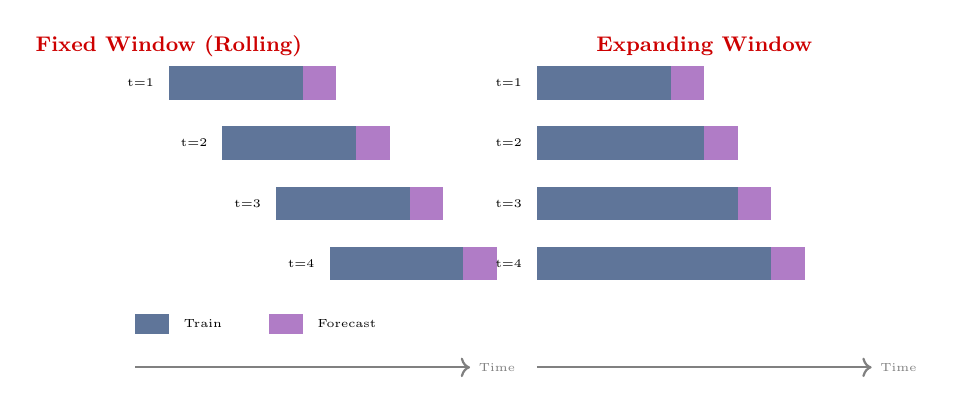
\begin{tikzpicture}[scale=0.85, transform shape]
        % Title for Fixed Window
        \node[font=\bfseries\small, color=IDAred] at (0, 3.8) {Fixed Window (Rolling)};

        % Fixed window iterations
        \foreach \i in {0,1,2,3} {
            \pgfmathsetmacro{\y}{3 - \i*0.9}
            \fill[MainBlue!70] ({\i*0.8}, \y) rectangle ({2+\i*0.8}, {\y+0.5});
            \fill[Purple!70] ({2+\i*0.8}, \y) rectangle ({2.5+\i*0.8}, {\y+0.5});
            \node[font=\tiny, left] at ({\i*0.8-0.1}, {\y+0.25}) {t=\pgfmathparse{int(\i+1)}\pgfmathresult};
        }
        \fill[MainBlue!70] (-0.5, -0.5) rectangle (0, -0.2);
        \node[font=\tiny, right] at (0.1, -0.35) {Train};
        \fill[Purple!70] (1.5, -0.5) rectangle (2, -0.2);
        \node[font=\tiny, right] at (2.1, -0.35) {Forecast};

        % Title for Expanding Window
        \node[font=\bfseries\small, color=IDAred] at (8, 3.8) {Expanding Window};

        % Expanding window iterations
        \foreach \i in {0,1,2,3} {
            \pgfmathsetmacro{\y}{3 - \i*0.9}
            \fill[MainBlue!70] (5.5, \y) rectangle ({7.5+\i*0.5}, {\y+0.5});
            \fill[Purple!70] ({7.5+\i*0.5}, \y) rectangle ({8+\i*0.5}, {\y+0.5});
            \node[font=\tiny, left] at (5.4, {\y+0.25}) {t=\pgfmathparse{int(\i+1)}\pgfmathresult};
        }

        \draw[->, thick, color=MediumGray] (-0.5, -1) -- (4.5, -1) node[right, font=\tiny] {Time};
        \draw[->, thick, color=MediumGray] (5.5, -1) -- (10.5, -1) node[right, font=\tiny] {Time};
    \end{tikzpicture}
    \end{center}
    \begin{block}{Comparison}
        \begin{itemize}\setlength{\itemsep}{0pt}
            \item \textbf{Fixed}: Window slides forward, constant size --- adapts to regime changes
            \item \textbf{Expanding}: Window grows over time --- uses all historical data
        \end{itemize}
    \end{block}
\end{frame}

\begin{frame}{1-Step vs Multi-Step Forecasting}
    \begin{columns}[T]
        \begin{column}{0.48\textwidth}
            \begin{block}{1-Step Ahead (Recursive)}
                \begin{itemize}\setlength{\itemsep}{1pt}
                    \item Forecast only next period
                    \begin{itemize}\setlength{\itemsep}{0pt}
                        \item Refit model after each step
                        \item Use actual value once revealed
                    \end{itemize}
                    \item Most accurate for short horizons
                \end{itemize}
            \end{block}
        \end{column}
        \begin{column}{0.48\textwidth}
            \begin{block}{Multi-Step (Direct)}
                \begin{itemize}\setlength{\itemsep}{1pt}
                    \item Forecast multiple periods ahead
                    \begin{itemize}\setlength{\itemsep}{0pt}
                        \item No refit between steps
                        \item Uses forecasted values as inputs
                    \end{itemize}
                    \item Uncertainty compounds over horizon
                \end{itemize}
            \end{block}
        \end{column}
    \end{columns}
    \vspace{0.3cm}
    \begin{center}
    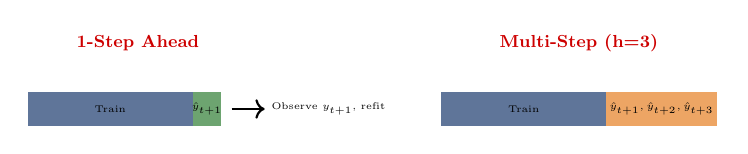
\begin{tikzpicture}[scale=0.7, transform shape]
        \node[font=\small\bfseries, color=IDAred] at (0, 1.5) {1-Step Ahead};
        \fill[MainBlue!70] (-2, 0) rectangle (1, 0.6);
        \fill[Forest!70] (1, 0) rectangle (1.5, 0.6);
        \node[font=\tiny] at (-0.5, 0.3) {Train};
        \node[font=\tiny] at (1.25, 0.3) {$\hat{y}_{t+1}$};
        \draw[->, thick] (1.7, 0.3) -- (2.3, 0.3);
        \node[font=\tiny, right] at (2.3, 0.3) {Observe $y_{t+1}$, refit};

        \node[font=\small\bfseries, color=IDAred] at (8, 1.5) {Multi-Step (h=3)};
        \fill[MainBlue!70] (5.5, 0) rectangle (8.5, 0.6);
        \fill[Orange!70] (8.5, 0) rectangle (10.5, 0.6);
        \node[font=\tiny] at (7, 0.3) {Train};
        \node[font=\tiny] at (9.5, 0.3) {$\hat{y}_{t+1}, \hat{y}_{t+2}, \hat{y}_{t+3}$};
    \end{tikzpicture}
    \end{center}
\end{frame}

\begin{frame}{Rolling Forecast: Step-by-Step Example}
    \begin{cminipage}{0.95\textwidth}
    {\small
    \begin{exampleblock}{Setup: ARIMA(1,1,0) with $\phi_1 = 0.6$}
        Model: $\Delta Y_t = \phi_1 \Delta Y_{t-1} + \varepsilon_t$ where $\Delta Y_t = Y_t - Y_{t-1}$
    \end{exampleblock}

    \vspace{0.1cm}

    \begin{block}{Given Data at Time $T$}
        $Y_{T-2} = 100$, \quad $Y_{T-1} = 103$, \quad $Y_T = 108$ \quad $\Rightarrow$ \quad $\Delta Y_{T-1} = 3$, \quad $\Delta Y_T = 5$
    \end{block}

    \vspace{0.1cm}

    \begin{alertblock}{1-Step Ahead Point Forecast}
        \begin{align*}
            \hat{\Delta Y}_{T+1|T} &= \phi_1 \cdot \Delta Y_T = 0.6 \times 5 = 3 \\[-0.2cm]
            \hat{Y}_{T+1|T} &= Y_T + \hat{\Delta Y}_{T+1|T} = 108 + 3 = \boxed{111}
        \end{align*}
    \end{alertblock}
    }
    \end{cminipage}
\end{frame}

\begin{frame}{Multi-Step Point Forecasts}
    \begin{cminipage}{0.95\textwidth}
    {\small
    \begin{block}{2-Step Ahead Forecast}
        \begin{align*}
            \hat{\Delta Y}_{T+2|T} &= \phi_1 \cdot \hat{\Delta Y}_{T+1|T} = 0.6 \times 3 = 1.8 \\[-0.2cm]
            \hat{Y}_{T+2|T} &= \hat{Y}_{T+1|T} + \hat{\Delta Y}_{T+2|T} = 111 + 1.8 = \boxed{112.8}
        \end{align*}
    \end{block}

    \vspace{0.05cm}

    \begin{block}{General Formula for $h$-Step Forecast (ARIMA(1,1,0))}
        \begin{align*}
            \hat{\Delta Y}_{T+h|T} &= \phi_1^h \cdot \Delta Y_T \\[-0.2cm]
            \hat{Y}_{T+h|T} &= Y_T + \Delta Y_T \cdot \frac{\phi_1(1-\phi_1^h)}{1-\phi_1}
        \end{align*}
    \end{block}

    \vspace{0.05cm}

    \begin{exampleblock}{Numerical: 3-Step Forecast}
        $\hat{Y}_{T+3|T} = 108 + 5 \times \frac{0.6(1-0.6^3)}{1-0.6} = 108 + 5 \times 1.092 = \boxed{113.46}$
    \end{exampleblock}
    }
    \end{cminipage}
\end{frame}

\begin{frame}{Confidence Intervals: Formulas}
    \begin{cminipage}{0.95\textwidth}
    {\small
    \begin{block}{Forecast Error Variance}
        For ARIMA(1,1,0), the $h$-step forecast error variance:
        $$\Var(e_{T+h|T}) = \sigma^2 \left(1 + \sum_{j=1}^{h-1} \psi_j^2 \right)$$
        where $\psi_j = \phi_1^{j-1}(1 + \phi_1 + \cdots + \phi_1^{j-1}) = \phi_1^{j-1} \cdot \frac{1-\phi_1^j}{1-\phi_1}$
    \end{block}

    \vspace{0.1cm}

    \begin{alertblock}{$(1-\alpha)$\% Confidence Interval}
        $$\hat{Y}_{T+h|T} \pm z_{\alpha/2} \cdot \sqrt{\Var(e_{T+h|T})}$$
        For 95\% CI: $z_{0.025} = 1.96$
    \end{alertblock}
    }
    \end{cminipage}
\end{frame}

\begin{frame}{Confidence Interval: Numerical Example}
    \vspace{-0.2cm}
    \begin{cminipage}{0.95\textwidth}
    {\small
    \begin{exampleblock}{Given: $\sigma^2 = 4$, $\phi_1 = 0.6$, $\hat{Y}_{T+1|T} = 111$}
    \end{exampleblock}

    \vspace{0.05cm}

    \begin{block}{1-Step Ahead CI}
        \begin{align*}
            \Var(e_{T+1|T}) &= \sigma^2 = 4 \\[-0.2cm]
            \text{95\% CI} &= 111 \pm 1.96 \times \sqrt{4} = 111 \pm 3.92 = \boxed{[107.08, \; 114.92]}
        \end{align*}
    \end{block}

    \vspace{0.05cm}

    \begin{block}{2-Step Ahead CI (for $\hat{Y}_{T+2|T} = 112.8$)}
        \begin{align*}
            \psi_1 &= 1 + \phi_1 = 1.6, \quad \Var(e_{T+2|T}) = 4(1 + 1.6^2) = 14.24 \\[-0.2cm]
            \text{95\% CI} &= 112.8 \pm 1.96 \times \sqrt{14.24} = 112.8 \pm 7.40 = \boxed{[105.40, \; 120.20]}
        \end{align*}
    \end{block}

    \textbf{Note}: CI widens as horizon increases!
    }
    \end{cminipage}
\end{frame}

\begin{frame}{Rolling Window Illustration}
    \vspace{-0.2cm}
    \begin{center}
        \includegraphics[width=0.95\textwidth, height=0.55\textheight, keepaspectratio]{ch3_rolling_forecast.pdf}
    \end{center}
    \vspace{-0.2cm}
    {\footnotesize
    \begin{block}{Rolling Procedure}
        \begin{itemize}\setlength{\itemsep}{0pt}
            \item Each window produces a 1-step ahead forecast
            \item Compare forecasts to actuals to compute RMSE, MAE
            \item Rolling window keeps model estimation up-to-date
        \end{itemize}
    \end{block}
    }
    \quantlet{TSA\_ch3\_rolling\_forecast}{https://github.com/QuantLet/TSA/tree/main/TSA_ch3/TSA_ch3_rolling_forecast}
\end{frame}

%=============================================================================
% CASE STUDY: REAL DATA
%=============================================================================
\section{Case Study}

\begin{frame}{Case Study: Complete ARIMA Analysis}
    \vspace{-0.4cm}
    \begin{cminipage}{0.95\textwidth}
    {\small
    \begin{block}{Objective}
        \begin{itemize}\setlength{\itemsep}{0pt}
            \item Forecast US Real GDP using the Box-Jenkins methodology
        \end{itemize}
    \end{block}

    \begin{block}{Steps}
        \begin{enumerate}\setlength{\itemsep}{0pt}
            \item \textbf{Step 1}: Visualize data and check stationarity
            \item \textbf{Step 2}: Apply unit root tests (ADF, KPSS)
            \item \textbf{Step 3}: Difference if needed, identify $p$ and $q$
            \item \textbf{Step 4}: Estimate the ARIMA model
            \item \textbf{Step 5}: Model diagnostics
            \item \textbf{Step 6}: Generate forecasts with confidence intervals
            \item \textbf{Step 7}: Evaluate forecast accuracy
        \end{enumerate}
    \end{block}

    \begin{alertblock}{Data}
        \begin{itemize}\setlength{\itemsep}{0pt}
            \item US Real GDP (FRED: GDPC1), Quarterly, 1990Q1--2024Q2, $n = 138$
        \end{itemize}
    \end{alertblock}
    }
    \end{cminipage}
\end{frame}

\begin{frame}{Case Study: US Real GDP (FRED)}
    \vspace{-0.2cm}
    \begin{center}
        \includegraphics[width=0.95\textwidth, height=0.55\textheight, keepaspectratio]{ch3_case_raw_data.pdf}
    \end{center}
    \vspace{-0.2cm}
    {\footnotesize
    \begin{block}{Data: FRED GDPC1 (1960Q1--2024Q3)}
        Quarterly Real GDP, seasonally adjusted, billions of chained 2017 dollars. Non-stationary series with upward trend $\Rightarrow$ requires differencing.
    \end{block}
    }
    \quantlet{TSA\_ch3\_case\_raw\_data}{https://github.com/QuantLet/TSA/tree/main/TSA_ch3/TSA_ch3_case_raw_data}
\end{frame}

\begin{frame}{Step 1: ADF Test for Stationarity}
    \vspace{-0.2cm}
    \begin{center}
        \includegraphics[width=0.95\textwidth, height=0.55\textheight, keepaspectratio]{ch3_case_adf_test.pdf}
    \end{center}
    \vspace{-0.2cm}
    {\footnotesize
    \begin{alertblock}{ADF Test Results}
        \textbf{Original series}: Large p-value $\Rightarrow$ fail to reject $H_0$ (unit root present).
        \textbf{First difference}: p-value $< 0.01$ $\Rightarrow$ reject $H_0$ $\Rightarrow$ $d = 1$ is sufficient.
    \end{alertblock}
    }
    \quantlet{TSA\_ch3\_case\_adf\_test}{https://github.com/QuantLet/TSA/tree/main/TSA_ch3/TSA_ch3_case_adf_test}
\end{frame}

\begin{frame}{Step 2: ACF/PACF Before and After Differencing}
    \vspace{-0.2cm}
    \begin{center}
        \includegraphics[width=0.95\textwidth, height=0.55\textheight, keepaspectratio]{ch3_case_acf_diff.pdf}
    \end{center}
    \vspace{-0.2cm}
    {\footnotesize
    \begin{exampleblock}{ACF/PACF Analysis}
        Top: Slow ACF decay (non-stationary) | Bottom: After differencing, low-order ARMA
    \end{exampleblock}
    }
    \quantlet{TSA\_ch3\_case\_acf\_diff}{https://github.com/QuantLet/TSA/tree/main/TSA_ch3/TSA_ch3_case_acf_diff}
\end{frame}

\begin{frame}{Step 3: ARIMA Model Comparison}
    \vspace{-0.2cm}
    \begin{center}
        \includegraphics[width=0.95\textwidth, height=0.55\textheight, keepaspectratio]{ch3_case_model_comparison.pdf}
    \end{center}
    \vspace{-0.2cm}
    {\footnotesize
    \begin{block}{Model Selection}
        Compare ARIMA(0,1,0), ARIMA(1,1,0), ARIMA(0,1,1), ARIMA(1,1,1). The model with lowest AIC is selected.
    \end{block}
    }
    \quantlet{TSA\_ch3\_case\_model\_comparison}{https://github.com/QuantLet/TSA/tree/main/TSA_ch3/TSA_ch3_case_model_comparison}
\end{frame}

\begin{frame}{Step 4: Diagnostic Checking}
    \vspace{-0.2cm}
    \begin{center}
        \includegraphics[width=0.95\textwidth, height=0.55\textheight, keepaspectratio]{ch3_case_diagnostics.pdf}
    \end{center}
    \vspace{-0.2cm}
    {\footnotesize
    \begin{alertblock}{ARIMA(1,1,1) Diagnostics}
        ACF: no autocorrelation $\checkmark$ \quad Q-Q: \textbf{non-normal} (COVID-19 outlier) \quad JB test: p $<$ 0.001
    \end{alertblock}
    }
    \quantlet{TSA\_ch3\_case\_diagnostics}{https://github.com/QuantLet/TSA/tree/main/TSA_ch3/TSA_ch3_case_diagnostics}
\end{frame}

\begin{frame}{Step 5: Out-of-Sample Forecasting}
    \vspace{-0.2cm}
    \begin{center}
        \includegraphics[width=0.95\textwidth, height=0.55\textheight, keepaspectratio]{ch3_case_forecast.pdf}
    \end{center}
    \vspace{-0.2cm}
    {\footnotesize
    \begin{block}{Train/Val/Test Split (70\%/15\%/15\%)}
        \textbf{Train 70\%} (blue): Estimation | \textbf{Val 15\%} (green): Tuning | \textbf{Test 15\%} (purple): Evaluation with 95\% CI
    \end{block}
    }
    \quantlet{TSA\_ch3\_case\_forecast}{https://github.com/QuantLet/TSA/tree/main/TSA_ch3/TSA_ch3_case_forecast}
\end{frame}

\begin{frame}{Step 6: Rolling Forecast with Train/Val/Test}
    \vspace{-0.2cm}
    \begin{center}
        \includegraphics[width=0.95\textwidth, height=0.55\textheight, keepaspectratio]{ch3_case_rolling_forecast.pdf}
    \end{center}
    \vspace{-0.2cm}
    {\footnotesize
    \begin{block}{Rolling 1-Step Ahead Forecast (Expanding Window, 95\% CI)}
        Train 70\% $\to$ Val 15\% $\to$ Test 15\% | Expanding window refits model at each step
    \end{block}
    }
    \quantlet{TSA\_ch3\_case\_rolling\_forecast}{https://github.com/QuantLet/TSA/tree/main/TSA_ch3/TSA_ch3_case_rolling_forecast}
\end{frame}

%=============================================================================
% SECTION 10: SUMMARY
%=============================================================================
\section{Summary}

\begin{frame}{Summary}
    \begin{cminipage}{0.95\textwidth}
    {\small
    \begin{block}{What we learned in this chapter}
        \begin{itemize}\setlength{\itemsep}{1pt}
            \item Non-stationarity in time series
            \begin{itemize}\setlength{\itemsep}{0pt}
                \item Deterministic vs stochastic trend; consequences for statistical inference
            \end{itemize}
            \item Differencing and integrated processes
            \begin{itemize}\setlength{\itemsep}{0pt}
                \item $\Delta Y_t = Y_t - Y_{t-1}$; if $Y_t \sim I(d)$, then $\Delta^d Y_t \sim I(0)$
            \end{itemize}
            \item ARIMA($p,d,q$) models and unit root tests
            \begin{itemize}\setlength{\itemsep}{0pt}
                \item ADF, PP, KPSS; Box-Jenkins: identify $\rightarrow$ estimate $\rightarrow$ validate
            \end{itemize}
            \item Forecasts with confidence intervals
            \begin{itemize}\setlength{\itemsep}{0pt}
                \item For I(1): CIs widen without bound ($\propto \sqrt{h}$)
            \end{itemize}
        \end{itemize}
    \end{block}
    \begin{exampleblock}{Key Insight}
        \begin{itemize}\setlength{\itemsep}{0pt}
            \item \textbf{Difference carefully}: One difference is usually sufficient ($d=1$). Over-differencing creates artificial autocorrelation.
        \end{itemize}
    \end{exampleblock}
    }
    \end{cminipage}
\end{frame}

%=============================================================================
\section{AI Use Case}
%=============================================================================

\begin{frame}{AI Exercise: Critical Thinking}
    \begin{cminipage}{0.95\textwidth}
    {\small
    \begin{block}{\footnotesize Prompt to test in ChatGPT / Claude / Copilot}
        ``I have a quarterly GDP time series (80 observations). Test stationarity, difference if needed, estimate an ARIMA model, and forecast 8 quarters ahead. Give me complete Python code with plots.''
    \end{block}
    \textbf{Exercise}:
    \begin{enumerate}\setlength{\itemsep}{0pt}
        \item Run the prompt in an LLM of your choice and critically analyze the response.
        \item Does it test stationarity with ADF \textit{before} estimating ARIMA? Does it also use KPSS?
        \item How does it determine the differencing order $d$? Does it check for over-differencing?
        \item How does it choose $p$ and $q$? ACF/PACF or just auto\_arima?
        \item Do forecast confidence intervals widen with horizon? (key I(1) property)
    \end{enumerate}
    \begin{alertblock}{}
        {\footnotesize \textbf{Warning}: AI-generated code may run without errors and look professional. \textit{That does not mean it is correct.}}
    \end{alertblock}
    }
    \end{cminipage}
\end{frame}

\begin{frame}{Quick Quiz}
    \begin{cminipage}{0.95\textwidth}
    {\small
    \begin{block}{Test your knowledge}
        \begin{itemize}\setlength{\itemsep}{4pt}
            \item[\textcolor{MainBlue}{\textbf{1.}}] What types of non-stationarity do you know and how is each treated?
            \item[\textcolor{MainBlue}{\textbf{2.}}] Why does random walk variance grow with time?
            \item[\textcolor{MainBlue}{\textbf{3.}}] What is the difference between ADF and KPSS tests?
            \item[\textcolor{MainBlue}{\textbf{4.}}] What happens if we over-difference a series?
            \item[\textcolor{MainBlue}{\textbf{5.}}] Why do ARIMA confidence intervals widen without bound for I(1) series?
        \end{itemize}
    \end{block}
    }
    \end{cminipage}
\end{frame}

\begin{frame}{Quiz Answers}
    \begin{cminipage}{0.95\textwidth}
    {\footnotesize
    \begin{exampleblock}{Answers}
        \begin{itemize}\setlength{\itemsep}{1pt}
            \item[\textcolor{MainBlue}{\textbf{1.}}] \textbf{Types}: Deterministic trend (regression); stochastic trend/unit root (differencing)
            \item[\textcolor{MainBlue}{\textbf{2.}}] \textbf{Variance}: $Y_t = \sum_{i=1}^t \varepsilon_i$ $\Rightarrow$ $\Var(Y_t) = t\sigma^2$ (shocks accumulate)
            \item[\textcolor{MainBlue}{\textbf{3.}}] \textbf{ADF vs KPSS}: ADF: $H_0$ = unit root; KPSS: $H_0$ = stationary. Used as complements.
            \item[\textcolor{MainBlue}{\textbf{4.}}] \textbf{Over-differencing}: Creates artificial negative autocorrelation ($\rho_1 \approx -0.5$); non-invertible MA(1)
            \item[\textcolor{MainBlue}{\textbf{5.}}] \textbf{Unbounded CIs}: $\Var(e_{T+h}) = \sigma^2 \sum_{j=0}^{h-1} \psi_j^2 \to \infty$ because $\psi_j$ do not decay
        \end{itemize}
    \end{exampleblock}
    }
    \end{cminipage}
\end{frame}

\begin{frame}{What's Next?}
    \begin{cminipage}{0.95\textwidth}
    \begin{center}
    \begin{minipage}{0.85\textwidth}
    \begin{block}{Chapter 4: SARIMA Models for Seasonal Data}
        \begin{itemize}\setlength{\itemsep}{0pt}
            \item \textbf{Seasonality}: repetitive patterns at regular intervals
            \item \textbf{Seasonal differencing}: the $(1-L^s)$ operator
            \item \textbf{SARIMA($p,d,q$)($P,D,Q$)$_s$}: seasonal extension of ARIMA
            \item \textbf{Model identification}: seasonal ACF/PACF
            \item \textbf{Case study}: Airline passengers forecast
        \end{itemize}
    \end{block}
    \end{minipage}
    \end{center}

    \vspace{0.3cm}
    \begin{center}
        \Large\textcolor{MainBlue}{Questions?}
    \end{center}
    \end{cminipage}
\end{frame}

%=============================================================================
% SECTION 11: QUIZ
%=============================================================================
\section{Quiz}

\begin{frame}{Question 1}
    \begin{cminipage}{0.95\textwidth}
    \begin{alertblock}{Question}
        \begin{itemize}\setlength{\itemsep}{0pt}
            \item A time series $Y_t$ follows a random walk: $Y_t = Y_{t-1} + \varepsilon_t$. What is $\Var(Y_t)$?
        \end{itemize}
    \end{alertblock}

    \vspace{0.3cm}

    \begin{block}{Answer Choices}

        \textcolor{MainBlue}{\textbf{(A)}} $\sigma^2$ (constant)\\[3pt]

        \textcolor{MainBlue}{\textbf{(B)}} $t \cdot \sigma^2$ (grows linearly with time)\\[3pt]

        \textcolor{MainBlue}{\textbf{(C)}} $\sigma^2 / t$ (decreases with time)\\[3pt]

        \textcolor{MainBlue}{\textbf{(D)}} $\sigma^{2t}$ (grows exponentially)

    \end{block}
    \end{cminipage}
\end{frame}

\begin{frame}{Question 1: Answer}
    \begin{cminipage}{0.95\textwidth}
    \vspace{-0.2cm}
    \begin{center}
        \includegraphics[width=0.98\textwidth, height=0.58\textheight, keepaspectratio]{ch3_quiz1_rw_variance.pdf}
    \end{center}
    \vspace{-3mm}
    {\small
    \begin{exampleblock}{Answer: (B)}
    \begin{itemize}\setlength{\itemsep}{0pt}
        \item Random walk variance grows linearly with time --- this is why random walks are non-stationary.
    \end{itemize}
    \end{exampleblock}
    }
    \hfill\quantlet{TSA\_ch3\_quiz1\_rw\_variance}{https://github.com/QuantLet/TSA/tree/main/TSA_ch3/TSA_ch3_quiz1_rw_variance}
    \end{cminipage}
\end{frame}

\begin{frame}{Question 2}
    \begin{cminipage}{0.95\textwidth}
    \begin{alertblock}{Question}
        \begin{itemize}\setlength{\itemsep}{0pt}
            \item If a series $Y_t$ is I(2), how many times must you difference it to achieve stationarity?
        \end{itemize}
    \end{alertblock}

    \vspace{0.3cm}

    \begin{block}{Answer Choices}

        \textcolor{MainBlue}{\textbf{(A)}} 0 times (already stationary)\\[3pt]

        \textcolor{MainBlue}{\textbf{(B)}} 1 time\\[3pt]

        \textcolor{MainBlue}{\textbf{(C)}} 2 times\\[3pt]

        \textcolor{MainBlue}{\textbf{(D)}} Cannot be made stationary by differencing

    \end{block}
    \end{cminipage}
\end{frame}

\begin{frame}{Question 2: Answer}
    \begin{cminipage}{0.95\textwidth}
    \vspace{-0.2cm}
    \begin{center}
        \includegraphics[width=0.98\textwidth, height=0.58\textheight, keepaspectratio]{ch3_quiz2_differencing.pdf}
    \end{center}
    \vspace{-3mm}
    {\small
    \begin{exampleblock}{Answer: (C)}
    \begin{itemize}\setlength{\itemsep}{0pt}
        \item I($d$) means ``integrated of order $d$'' --- requires $d$ differences for stationarity.
    \end{itemize}
    \end{exampleblock}
    }
    \hfill\quantlet{TSA\_ch3\_quiz2\_differencing}{https://github.com/QuantLet/TSA/tree/main/TSA_ch3/TSA_ch3_quiz2_differencing}
    \end{cminipage}
\end{frame}

\begin{frame}{Question 3}
    \begin{cminipage}{0.95\textwidth}
    \begin{alertblock}{Question}
        \begin{itemize}\setlength{\itemsep}{0pt}
            \item You run an ADF test and get a test statistic of $-2.1$ with critical values: $-3.43$ (1\%), $-2.86$ (5\%), $-2.57$ (10\%). What do you conclude?
        \end{itemize}
    \end{alertblock}

    \vspace{0.3cm}

    \begin{block}{Answer Choices}

        \textcolor{MainBlue}{\textbf{(A)}} Reject $H_0$: series is stationary at all levels\\[3pt]

        \textcolor{MainBlue}{\textbf{(B)}} Reject $H_0$: series is stationary at 10\% level only\\[3pt]

        \textcolor{MainBlue}{\textbf{(C)}} Fail to reject $H_0$: series likely has a unit root\\[3pt]

        \textcolor{MainBlue}{\textbf{(D)}} The test is inconclusive

    \end{block}
    \end{cminipage}
\end{frame}

\begin{frame}{Question 3: Answer}
    \begin{cminipage}{0.95\textwidth}
    \vspace{-0.2cm}
    \begin{center}
        \includegraphics[width=0.98\textwidth, height=0.58\textheight, keepaspectratio]{ch3_quiz3_adf_test.pdf}
    \end{center}
    \vspace{-3mm}
    {\small
    \begin{exampleblock}{Answer: (C)}
    \begin{itemize}\setlength{\itemsep}{0pt}
        \item Test stat $-2.1 > -2.57$ (10\% CV) $\Rightarrow$ Cannot reject at any level. Consider differencing.
    \end{itemize}
    \end{exampleblock}
    }
    \hfill\quantlet{TSA\_ch3\_quiz3\_adf\_test}{https://github.com/QuantLet/TSA/tree/main/TSA_ch3/TSA_ch3_quiz3_adf_test}
    \end{cminipage}
\end{frame}

\begin{frame}{Question 4}
    \begin{cminipage}{0.95\textwidth}
    \begin{alertblock}{Question}
        \begin{itemize}\setlength{\itemsep}{0pt}
            \item For an ARIMA(1,1,0) model, what is the ACF pattern of the \textbf{differenced} series $\Delta Y_t$?
        \end{itemize}
    \end{alertblock}

    \vspace{0.3cm}

    \begin{block}{Answer Choices}

        \textcolor{MainBlue}{\textbf{(A)}} Cuts off after lag 1\\[3pt]

        \textcolor{MainBlue}{\textbf{(B)}} Decays exponentially\\[3pt]

        \textcolor{MainBlue}{\textbf{(C)}} Alternates in sign\\[3pt]

        \textcolor{MainBlue}{\textbf{(D)}} Is zero at all lags

    \end{block}
    \end{cminipage}
\end{frame}

\begin{frame}{Question 4: Answer}
    \begin{cminipage}{0.95\textwidth}
    \vspace{-0.2cm}
    \begin{center}
        \includegraphics[width=0.98\textwidth, height=0.58\textheight, keepaspectratio]{ch3_quiz4_acf_decay.pdf}
    \end{center}
    \vspace{-3mm}
    {\small
    \begin{exampleblock}{Answer: (B)}
    \begin{itemize}\setlength{\itemsep}{0pt}
        \item ARIMA(1,1,0) $\Rightarrow$ $\Delta Y_t$ follows AR(1) with ACF $\rho_k = \phi_1^k$ (geometric decay).
    \end{itemize}
    \end{exampleblock}
    }
    \hfill\quantlet{TSA\_ch3\_quiz4\_acf\_decay}{https://github.com/QuantLet/TSA/tree/main/TSA_ch3/TSA_ch3_quiz4_acf_decay}
    \end{cminipage}
\end{frame}

\begin{frame}{Question 5}
    \begin{cminipage}{0.95\textwidth}
    \begin{alertblock}{Question}
        \begin{itemize}\setlength{\itemsep}{0pt}
            \item What happens to ARIMA forecast confidence intervals as the horizon $h$ increases for an I(1) series?
        \end{itemize}
    \end{alertblock}

    \vspace{0.3cm}

    \begin{block}{Answer Choices}

        \textcolor{MainBlue}{\textbf{(A)}} They stay constant\\[3pt]

        \textcolor{MainBlue}{\textbf{(B)}} They narrow (more precision)\\[3pt]

        \textcolor{MainBlue}{\textbf{(C)}} They widen without bound\\[3pt]

        \textcolor{MainBlue}{\textbf{(D)}} They widen but converge to a limit

    \end{block}
    \end{cminipage}
\end{frame}

\begin{frame}{Question 5: Answer}
    \begin{cminipage}{0.95\textwidth}
    \vspace{-0.2cm}
    \begin{center}
        \includegraphics[width=0.98\textwidth, height=0.58\textheight, keepaspectratio]{ch3_quiz5_forecast_ci.pdf}
    \end{center}
    \vspace{-3mm}
    {\small
    \begin{exampleblock}{Answer: (C)}
    \begin{itemize}\setlength{\itemsep}{0pt}
        \item For I(1): CI width $\propto \sqrt{h}$ (unbounded). For I(0): CIs converge to a limit.
    \end{itemize}
    \end{exampleblock}
    }
    \hfill\quantlet{TSA\_ch3\_quiz5\_forecast\_ci}{https://github.com/QuantLet/TSA/tree/main/TSA_ch3/TSA_ch3_quiz5_forecast_ci}
    \end{cminipage}
\end{frame}

\begin{frame}{Bibliography I}
    \begin{cminipage}{0.95\textwidth}
    {\small
    \begin{block}{Unit Root Tests}
        \begin{itemize}
            \item Dickey, D.A., \& Fuller, W.A. (1979). Distribution of the Estimators for Autoregressive Time Series with a Unit Root, \textit{JASA}, 74(366), 427--431.
            \item Phillips, P.C.B., \& Perron, P. (1988). Testing for a Unit Root in Time Series Regression, \textit{Biometrika}, 75(2), 335--346.
            \item Kwiatkowski, D., Phillips, P.C.B., Schmidt, P., \& Shin, Y. (1992). Testing the Null Hypothesis of Stationarity, \textit{Journal of Econometrics}, 54(1-3), 159--178.
        \end{itemize}
    \end{block}

    \begin{exampleblock}{ARIMA Models and Automatic Selection}
        \begin{itemize}
            \item Box, G.E.P., \& Jenkins, G.M. (1970). \textit{Time Series Analysis: Forecasting and Control}, Holden-Day.
            \item Hyndman, R.J., \& Khandakar, Y. (2008). Automatic Time Series Forecasting: The \texttt{forecast} Package for R, \textit{Journal of Statistical Software}, 27(3), 1--22.
        \end{itemize}
    \end{exampleblock}
    }
    \end{cminipage}
\end{frame}

\begin{frame}{Bibliography II}
    \begin{cminipage}{0.95\textwidth}
    {\small
    \begin{block}{Textbooks and Additional References}
        \begin{itemize}
            \item Hamilton, J.D. (1994). \textit{Time Series Analysis}, Princeton University Press.
            \item Shumway, R.H., \& Stoffer, D.S. (2017). \textit{Time Series Analysis and Its Applications}, 4th ed., Springer.
            \item Hyndman, R.J., \& Athanasopoulos, G. (2021). \textit{Forecasting: Principles and Practice}, 3rd ed., OTexts.
        \end{itemize}
    \end{block}

    \begin{exampleblock}{Online Resources and Code}
        \begin{itemize}
            \item \textbf{Quantlet}: \url{https://quantlet.com} $\rightarrow$ Code repository for statistics
            \item \textbf{Quantinar}: \url{https://quantinar.com} $\rightarrow$ Learning platform for quantitative methods
            \item \textbf{GitHub TSA}: \url{https://github.com/QuantLet/TSA/tree/main/TSA_ch3} $\rightarrow$ Python code for this chapter
        \end{itemize}
    \end{exampleblock}
    }
    \end{cminipage}
\end{frame}

\begin{frame}{}
    \begin{cminipage}{0.95\textwidth}
    \centering
    \Huge\textcolor{MainBlue}{Thank You!}

    \vspace{0.8cm}

    \Large Questions?

    \vspace{1cm}

    \normalsize
    Course materials available at: \url{https://danpele.github.io/Time-Series-Analysis/}

    \vspace{0.3cm}

    \href{https://quantlet.com}{\raisebox{-0.15em}{\includegraphics[height=0.8em]{ql_logo.png}} Quantlet} \hspace{0.5cm}
    \href{https://quantinar.com}{\raisebox{-0.15em}{\includegraphics[height=0.8em]{qr_logo.png}} Quantinar}
    \end{cminipage}
\end{frame}

\end{document}
